\documentclass[twoside]{book}

% Packages required by doxygen
\usepackage{calc}
\usepackage{doxygen}
\usepackage{graphicx}
\usepackage[utf8]{inputenc}
\usepackage{makeidx}
\usepackage{multicol}
\usepackage{multirow}
\usepackage{textcomp}
\usepackage[table]{xcolor}

% Font selection
\usepackage[T1]{fontenc}
\usepackage{mathptmx}
\usepackage[scaled=.90]{helvet}
\usepackage{courier}
\usepackage{amssymb}
\usepackage{sectsty}
\renewcommand{\familydefault}{\sfdefault}
\allsectionsfont{%
  \fontseries{bc}\selectfont%
  \color{darkgray}%
}
\renewcommand{\DoxyLabelFont}{%
  \fontseries{bc}\selectfont%
  \color{darkgray}%
}

% Page & text layout
\usepackage{geometry}
\geometry{%
  a4paper,%
  top=2.5cm,%
  bottom=2.5cm,%
  left=2.5cm,%
  right=2.5cm%
}
\tolerance=750
\hfuzz=15pt
\hbadness=750
\setlength{\emergencystretch}{15pt}
\setlength{\parindent}{0cm}
\setlength{\parskip}{0.2cm}
\makeatletter
\renewcommand{\paragraph}{%
  \@startsection{paragraph}{4}{0ex}{-1.0ex}{1.0ex}{%
    \normalfont\normalsize\bfseries\SS@parafont%
  }%
}
\renewcommand{\subparagraph}{%
  \@startsection{subparagraph}{5}{0ex}{-1.0ex}{1.0ex}{%
    \normalfont\normalsize\bfseries\SS@subparafont%
  }%
}
\makeatother

% Headers & footers
\usepackage{fancyhdr}
\pagestyle{fancyplain}
\fancyhead[LE]{\fancyplain{}{\bfseries\thepage}}
\fancyhead[CE]{\fancyplain{}{}}
\fancyhead[RE]{\fancyplain{}{\bfseries\leftmark}}
\fancyhead[LO]{\fancyplain{}{\bfseries\rightmark}}
\fancyhead[CO]{\fancyplain{}{}}
\fancyhead[RO]{\fancyplain{}{\bfseries\thepage}}
\fancyfoot[LE]{\fancyplain{}{}}
\fancyfoot[CE]{\fancyplain{}{}}
\fancyfoot[RE]{\fancyplain{}{\bfseries\scriptsize Generated on Sun Jan 17 2016 21\-:52\-:56 for My Project by Doxygen }}
\fancyfoot[LO]{\fancyplain{}{\bfseries\scriptsize Generated on Sun Jan 17 2016 21\-:52\-:56 for My Project by Doxygen }}
\fancyfoot[CO]{\fancyplain{}{}}
\fancyfoot[RO]{\fancyplain{}{}}
\renewcommand{\footrulewidth}{0.4pt}
\renewcommand{\chaptermark}[1]{%
  \markboth{#1}{}%
}
\renewcommand{\sectionmark}[1]{%
  \markright{\thesection\ #1}%
}

% Indices & bibliography
\usepackage{natbib}
\usepackage[titles]{tocloft}
\setcounter{tocdepth}{3}
\setcounter{secnumdepth}{5}
\makeindex

% Hyperlinks (required, but should be loaded last)
\usepackage{ifpdf}
\ifpdf
  \usepackage[pdftex,pagebackref=true]{hyperref}
\else
  \usepackage[ps2pdf,pagebackref=true]{hyperref}
\fi
\hypersetup{%
  colorlinks=true,%
  linkcolor=blue,%
  citecolor=blue,%
  unicode%
}

% Custom commands
\newcommand{\clearemptydoublepage}{%
  \newpage{\pagestyle{empty}\cleardoublepage}%
}


%===== C O N T E N T S =====

\begin{document}

% Titlepage & ToC
\hypersetup{pageanchor=false}
\pagenumbering{roman}
\begin{titlepage}
\vspace*{7cm}
\begin{center}%
{\Large My Project }\\
\vspace*{1cm}
{\large Generated by Doxygen 1.8.6}\\
\vspace*{0.5cm}
{\small Sun Jan 17 2016 21:52:56}\\
\end{center}
\end{titlepage}
\clearemptydoublepage
\tableofcontents
\clearemptydoublepage
\pagenumbering{arabic}
\hypersetup{pageanchor=true}

%--- Begin generated contents ---
\chapter{Main Page}
\label{index}\hypertarget{index}{}\input{index}
\chapter{Satellite\-\_\-\-Scheduler}
\label{md_README}
\hypertarget{md_README}{}
Prototype of the satellite scheduler used for the Electron Losses and Fields Investigation (E\-L\-F\-I\-N) Cube\-Sat

\subsection*{$\ast$$\ast$\-Overview\-:$\ast$$\ast$}

Module for creating / manipulating schedules for the satellites. Currently can create, store, edit, and constraint check a schedule. Logs all events, including user outputs, database manipulations, and user inputs in console window.

{\bfseries Open 'html / index.\-html' in a web browser for easily navigable in depth documentation.}



\subsection*{$\ast$$\ast$\-Running\-:$\ast$$\ast$}

Run {\itshape start.\-sh}. This will compile, run, and update existing documentation. Edit this file to include any new U\-I / Python files that need to be compiled.

\subsection*{$\ast$$\ast$\-Files by Type\-:$\ast$$\ast$}

When {\itshape start.\-sh} is run, user interface (.ui) files created by Qt Designer are compiled by pyuic into a format compatible with Py\-Qt. The files fall into these three formats as follows\-:

\subsubsection*{$\ast$$\ast$\-User Interface Layouts (.ui)$\ast$$\ast$}


\begin{DoxyItemize}
\item Add\-\_\-\-Activity\-\_\-\-Dialog.\-ui
\item E\-L\-F\-I\-N\-\_\-\-Proto.\-ui
\item Help\-\_\-\-Dialog.\-ui
\item Override\-\_\-\-Dialog.\-ui
\end{DoxyItemize}

\subsubsection*{$\ast$$\ast$\-Auto Generated by Pyuic (.py)$\ast$$\ast$}


\begin{DoxyItemize}
\item Add\-\_\-\-Activity\-\_\-\-Dialog.\-py
\item E\-L\-F\-I\-N\-\_\-\-Proto.\-py
\item Help\-\_\-\-Dialog.\-py
\item Override\-\_\-\-Dialog.\-py
\end{DoxyItemize}

\subsubsection*{$\ast$$\ast$\-User Created (.py)$\ast$$\ast$}


\begin{DoxyItemize}
\item Console\-I\-O.\-py
\item Constraints\-Checker.\-py
\item Database\-Classes.\-py
\item D\-B\-\_\-\-Manager.\-py
\item run\-E\-L\-F\-I\-N\-\_\-\-Proto.\-py
\item Scheduler.\-py
\item start.\-sh 
\end{DoxyItemize}
\chapter{Hierarchical Index}
\section{Class Hierarchy}
This inheritance list is sorted roughly, but not completely, alphabetically\-:\begin{DoxyCompactList}
\item \contentsline{section}{Database\-\_\-\-Classes.\-Activity}{\pageref{classDatabase__Classes_1_1Activity}}{}
\item \contentsline{section}{Console\-I\-O.\-Console\-I\-O}{\pageref{classConsoleIO_1_1ConsoleIO}}{}
\item \contentsline{section}{Constraints\-Checker.\-Constraints\-Checker}{\pageref{classConstraintsChecker_1_1ConstraintsChecker}}{}
\item \contentsline{section}{D\-B\-\_\-\-Manager.\-Database\-Manager}{\pageref{classDB__Manager_1_1DatabaseManager}}{}
\item object\begin{DoxyCompactList}
\item \contentsline{section}{Add\-\_\-\-Activity\-\_\-\-Dialog.\-Ui\-\_\-\-Add\-\_\-\-Activity\-\_\-\-Dialog}{\pageref{classAdd__Activity__Dialog_1_1Ui__Add__Activity__Dialog}}{}
\begin{DoxyCompactList}
\item \contentsline{section}{run\-E\-L\-F\-I\-N\-\_\-\-Proto.\-Add\-Activity\-Dialog}{\pageref{classrunELFIN__Proto_1_1AddActivityDialog}}{}
\end{DoxyCompactList}
\item \contentsline{section}{E\-L\-F\-I\-N\-\_\-\-Proto.\-Ui\-\_\-\-Main\-Window}{\pageref{classELFIN__Proto_1_1Ui__MainWindow}}{}
\begin{DoxyCompactList}
\item \contentsline{section}{run\-E\-L\-F\-I\-N\-\_\-\-Proto.\-My\-Main\-Window}{\pageref{classrunELFIN__Proto_1_1MyMainWindow}}{}
\end{DoxyCompactList}
\item \contentsline{section}{Help\-\_\-\-Dialog.\-Ui\-\_\-\-Dialog}{\pageref{classHelp__Dialog_1_1Ui__Dialog}}{}
\begin{DoxyCompactList}
\item \contentsline{section}{run\-E\-L\-F\-I\-N\-\_\-\-Proto.\-Help\-Dialog}{\pageref{classrunELFIN__Proto_1_1HelpDialog}}{}
\end{DoxyCompactList}
\item \contentsline{section}{Override\-\_\-\-Dialog.\-Ui\-\_\-\-Override\-\_\-\-Dialog}{\pageref{classOverride__Dialog_1_1Ui__Override__Dialog}}{}
\begin{DoxyCompactList}
\item \contentsline{section}{Console\-I\-O.\-Override\-\_\-\-Dialog}{\pageref{classConsoleIO_1_1Override__Dialog}}{}
\end{DoxyCompactList}
\end{DoxyCompactList}
\item Q\-Dialog\begin{DoxyCompactList}
\item \contentsline{section}{Console\-I\-O.\-Override\-\_\-\-Dialog}{\pageref{classConsoleIO_1_1Override__Dialog}}{}
\item \contentsline{section}{run\-E\-L\-F\-I\-N\-\_\-\-Proto.\-Add\-Activity\-Dialog}{\pageref{classrunELFIN__Proto_1_1AddActivityDialog}}{}
\item \contentsline{section}{run\-E\-L\-F\-I\-N\-\_\-\-Proto.\-Help\-Dialog}{\pageref{classrunELFIN__Proto_1_1HelpDialog}}{}
\end{DoxyCompactList}
\item Q\-Main\-Window\begin{DoxyCompactList}
\item \contentsline{section}{run\-E\-L\-F\-I\-N\-\_\-\-Proto.\-My\-Main\-Window}{\pageref{classrunELFIN__Proto_1_1MyMainWindow}}{}
\end{DoxyCompactList}
\item \contentsline{section}{Scheduler.\-Scheduler}{\pageref{classScheduler_1_1Scheduler}}{}
\end{DoxyCompactList}

\chapter{Class Index}
\section{Class List}
Here are the classes, structs, unions and interfaces with brief descriptions\-:\begin{DoxyCompactList}
\item\contentsline{section}{\hyperlink{classDatabase__Classes_1_1Activity}{Database\-\_\-\-Classes.\-Activity} }{\pageref{classDatabase__Classes_1_1Activity}}{}
\item\contentsline{section}{\hyperlink{classrunELFIN__Proto_1_1AddActivityDialog}{run\-E\-L\-F\-I\-N\-\_\-\-Proto.\-Add\-Activity\-Dialog} }{\pageref{classrunELFIN__Proto_1_1AddActivityDialog}}{}
\item\contentsline{section}{\hyperlink{classConsoleIO_1_1ConsoleIO}{Console\-I\-O.\-Console\-I\-O} }{\pageref{classConsoleIO_1_1ConsoleIO}}{}
\item\contentsline{section}{\hyperlink{classConstraintsChecker_1_1ConstraintsChecker}{Constraints\-Checker.\-Constraints\-Checker} }{\pageref{classConstraintsChecker_1_1ConstraintsChecker}}{}
\item\contentsline{section}{\hyperlink{classDB__Manager_1_1DatabaseManager}{D\-B\-\_\-\-Manager.\-Database\-Manager} }{\pageref{classDB__Manager_1_1DatabaseManager}}{}
\item\contentsline{section}{\hyperlink{classrunELFIN__Proto_1_1HelpDialog}{run\-E\-L\-F\-I\-N\-\_\-\-Proto.\-Help\-Dialog} }{\pageref{classrunELFIN__Proto_1_1HelpDialog}}{}
\item\contentsline{section}{\hyperlink{classrunELFIN__Proto_1_1MyMainWindow}{run\-E\-L\-F\-I\-N\-\_\-\-Proto.\-My\-Main\-Window} }{\pageref{classrunELFIN__Proto_1_1MyMainWindow}}{}
\item\contentsline{section}{\hyperlink{classConsoleIO_1_1Override__Dialog}{Console\-I\-O.\-Override\-\_\-\-Dialog} }{\pageref{classConsoleIO_1_1Override__Dialog}}{}
\item\contentsline{section}{\hyperlink{classScheduler_1_1Scheduler}{Scheduler.\-Scheduler} }{\pageref{classScheduler_1_1Scheduler}}{}
\item\contentsline{section}{\hyperlink{classAdd__Activity__Dialog_1_1Ui__Add__Activity__Dialog}{Add\-\_\-\-Activity\-\_\-\-Dialog.\-Ui\-\_\-\-Add\-\_\-\-Activity\-\_\-\-Dialog} }{\pageref{classAdd__Activity__Dialog_1_1Ui__Add__Activity__Dialog}}{}
\item\contentsline{section}{\hyperlink{classHelp__Dialog_1_1Ui__Dialog}{Help\-\_\-\-Dialog.\-Ui\-\_\-\-Dialog} }{\pageref{classHelp__Dialog_1_1Ui__Dialog}}{}
\item\contentsline{section}{\hyperlink{classELFIN__Proto_1_1Ui__MainWindow}{E\-L\-F\-I\-N\-\_\-\-Proto.\-Ui\-\_\-\-Main\-Window} }{\pageref{classELFIN__Proto_1_1Ui__MainWindow}}{}
\item\contentsline{section}{\hyperlink{classOverride__Dialog_1_1Ui__Override__Dialog}{Override\-\_\-\-Dialog.\-Ui\-\_\-\-Override\-\_\-\-Dialog} }{\pageref{classOverride__Dialog_1_1Ui__Override__Dialog}}{}
\end{DoxyCompactList}

\chapter{Class Documentation}
\hypertarget{classDatabase__Classes_1_1Activity}{\section{Database\-\_\-\-Classes.\-Activity Class Reference}
\label{classDatabase__Classes_1_1Activity}\index{Database\-\_\-\-Classes.\-Activity@{Database\-\_\-\-Classes.\-Activity}}
}
\subsection*{Public Member Functions}
\begin{DoxyCompactItemize}
\item 
\hypertarget{classDatabase__Classes_1_1Activity_a5017887db3b072677022ce35c3512a33}{def {\bfseries \-\_\-\-\_\-init\-\_\-\-\_\-}}\label{classDatabase__Classes_1_1Activity_a5017887db3b072677022ce35c3512a33}

\item 
\hypertarget{classDatabase__Classes_1_1Activity_a008a711f8035ce5790d9c85097c5748a}{def {\bfseries save\-\_\-state}}\label{classDatabase__Classes_1_1Activity_a008a711f8035ce5790d9c85097c5748a}

\item 
\hypertarget{classDatabase__Classes_1_1Activity_afecd5fb90df723c4b3f4b2ba7eee14cd}{def {\bfseries reset\-\_\-parameters\-\_\-from\-\_\-save}}\label{classDatabase__Classes_1_1Activity_afecd5fb90df723c4b3f4b2ba7eee14cd}

\item 
\hypertarget{classDatabase__Classes_1_1Activity_ae6ba07eeb9e023dc9109a18b1d58c0e9}{def {\bfseries get\-\_\-duration}}\label{classDatabase__Classes_1_1Activity_ae6ba07eeb9e023dc9109a18b1d58c0e9}

\item 
\hypertarget{classDatabase__Classes_1_1Activity_a803a0c548bb38dcfcd4af1dc399cc004}{def {\bfseries pretty\-\_\-string}}\label{classDatabase__Classes_1_1Activity_a803a0c548bb38dcfcd4af1dc399cc004}

\end{DoxyCompactItemize}
\subsection*{Public Attributes}
\begin{DoxyCompactItemize}
\item 
\hypertarget{classDatabase__Classes_1_1Activity_a4304d966ad1a565b353c37e221f8550a}{{\bfseries start\-Time}}\label{classDatabase__Classes_1_1Activity_a4304d966ad1a565b353c37e221f8550a}

\item 
\hypertarget{classDatabase__Classes_1_1Activity_a2dd5e500b88ceced9a749435fa6058b3}{{\bfseries stop\-Time}}\label{classDatabase__Classes_1_1Activity_a2dd5e500b88ceced9a749435fa6058b3}

\item 
\hypertarget{classDatabase__Classes_1_1Activity_a6ab830b6302d0a004977142fe18b0aff}{{\bfseries parameters}}\label{classDatabase__Classes_1_1Activity_a6ab830b6302d0a004977142fe18b0aff}

\item 
\hypertarget{classDatabase__Classes_1_1Activity_a41af32da7c5e4ce656188b809198d535}{{\bfseries thing}}\label{classDatabase__Classes_1_1Activity_a41af32da7c5e4ce656188b809198d535}

\item 
\hypertarget{classDatabase__Classes_1_1Activity_a71776c12e44d9f064f4c30a5a170ab9d}{{\bfseries saved\-\_\-start\-Time}}\label{classDatabase__Classes_1_1Activity_a71776c12e44d9f064f4c30a5a170ab9d}

\item 
\hypertarget{classDatabase__Classes_1_1Activity_a7e5e0fcdeae75539c0fcfc2a6788d69b}{{\bfseries saved\-\_\-stop\-Time}}\label{classDatabase__Classes_1_1Activity_a7e5e0fcdeae75539c0fcfc2a6788d69b}

\item 
\hypertarget{classDatabase__Classes_1_1Activity_ad16876c648873ca8bf1f0c6d13a79951}{{\bfseries saved\-\_\-parameters}}\label{classDatabase__Classes_1_1Activity_ad16876c648873ca8bf1f0c6d13a79951}

\item 
\hypertarget{classDatabase__Classes_1_1Activity_a7e6a413c84129b8b71839ee3a86c8bed}{{\bfseries duration}}\label{classDatabase__Classes_1_1Activity_a7e6a413c84129b8b71839ee3a86c8bed}

\end{DoxyCompactItemize}


The documentation for this class was generated from the following file\-:\begin{DoxyCompactItemize}
\item 
Database\-\_\-\-Classes.\-py\end{DoxyCompactItemize}

\hypertarget{classrunELFIN__Proto_1_1AddActivityDialog}{\section{run\-E\-L\-F\-I\-N\-\_\-\-Proto.\-Add\-Activity\-Dialog Class Reference}
\label{classrunELFIN__Proto_1_1AddActivityDialog}\index{run\-E\-L\-F\-I\-N\-\_\-\-Proto.\-Add\-Activity\-Dialog@{run\-E\-L\-F\-I\-N\-\_\-\-Proto.\-Add\-Activity\-Dialog}}
}


Activity dialog to display to edit/add activities.  


Inheritance diagram for run\-E\-L\-F\-I\-N\-\_\-\-Proto.\-Add\-Activity\-Dialog\-:\begin{figure}[H]
\begin{center}
\leavevmode
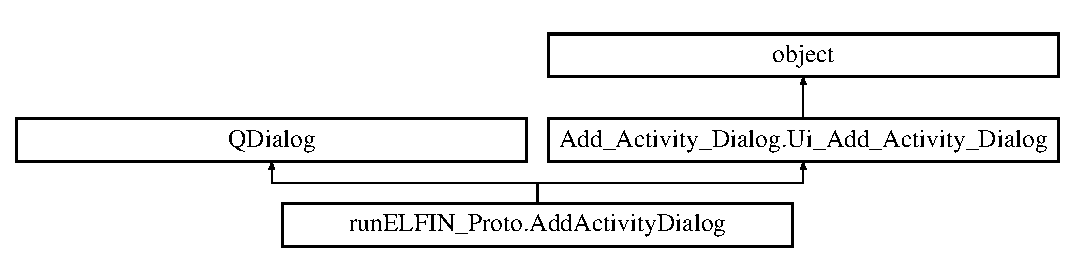
\includegraphics[height=3.000000cm]{classrunELFIN__Proto_1_1AddActivityDialog}
\end{center}
\end{figure}
\subsection*{Public Member Functions}
\begin{DoxyCompactItemize}
\item 
\hypertarget{classrunELFIN__Proto_1_1AddActivityDialog_a471b245c26d4148a8c9575e8ce075c5b}{def {\bfseries \-\_\-\-\_\-init\-\_\-\-\_\-}}\label{classrunELFIN__Proto_1_1AddActivityDialog_a471b245c26d4148a8c9575e8ce075c5b}

\item 
\hypertarget{classrunELFIN__Proto_1_1AddActivityDialog_a154107cc596262338c88ecd63713cef5}{def {\bfseries add\-\_\-activity}}\label{classrunELFIN__Proto_1_1AddActivityDialog_a154107cc596262338c88ecd63713cef5}

\item 
\hypertarget{classrunELFIN__Proto_1_1AddActivityDialog_a2dbd21f4cd94130413857ac9954fc325}{def {\bfseries add\-\_\-new\-\_\-activity\-\_\-item}}\label{classrunELFIN__Proto_1_1AddActivityDialog_a2dbd21f4cd94130413857ac9954fc325}

\item 
\hypertarget{classrunELFIN__Proto_1_1AddActivityDialog_a13af5c9e50240aa9b2ec22709ff4b8be}{def {\bfseries close}}\label{classrunELFIN__Proto_1_1AddActivityDialog_a13af5c9e50240aa9b2ec22709ff4b8be}

\end{DoxyCompactItemize}
\subsection*{Public Attributes}
\begin{DoxyCompactItemize}
\item 
\hypertarget{classrunELFIN__Proto_1_1AddActivityDialog_a12140c8cdceb2058b09160f7c7aab592}{{\bfseries parent}}\label{classrunELFIN__Proto_1_1AddActivityDialog_a12140c8cdceb2058b09160f7c7aab592}

\item 
\hypertarget{classrunELFIN__Proto_1_1AddActivityDialog_a7c13e3ec59ccf680918b02899fe94660}{{\bfseries parent\-\_\-layout}}\label{classrunELFIN__Proto_1_1AddActivityDialog_a7c13e3ec59ccf680918b02899fe94660}

\item 
\hypertarget{classrunELFIN__Proto_1_1AddActivityDialog_a896da045d7da424e13a0c7505d186965}{{\bfseries scheduler}}\label{classrunELFIN__Proto_1_1AddActivityDialog_a896da045d7da424e13a0c7505d186965}

\item 
\hypertarget{classrunELFIN__Proto_1_1AddActivityDialog_aa0a22cfdc9dca4b2220d3923d6c221fa}{{\bfseries base\-\_\-x\-\_\-position}}\label{classrunELFIN__Proto_1_1AddActivityDialog_aa0a22cfdc9dca4b2220d3923d6c221fa}

\item 
\hypertarget{classrunELFIN__Proto_1_1AddActivityDialog_aea0b78ce5f90cb87257f35789943b4ff}{{\bfseries base\-\_\-y\-\_\-position}}\label{classrunELFIN__Proto_1_1AddActivityDialog_aea0b78ce5f90cb87257f35789943b4ff}

\item 
\hypertarget{classrunELFIN__Proto_1_1AddActivityDialog_a727e08a9d43c339ec2215bf86c9930ad}{{\bfseries base\-\_\-x\-\_\-line\-\_\-distance}}\label{classrunELFIN__Proto_1_1AddActivityDialog_a727e08a9d43c339ec2215bf86c9930ad}

\item 
\hypertarget{classrunELFIN__Proto_1_1AddActivityDialog_a8715c0edf9b15b098652d7fd53620605}{{\bfseries base\-\_\-y\-\_\-line\-\_\-distance}}\label{classrunELFIN__Proto_1_1AddActivityDialog_a8715c0edf9b15b098652d7fd53620605}

\item 
\hypertarget{classrunELFIN__Proto_1_1AddActivityDialog_a1e40557c0232af6ed9a6b4ed521733e5}{{\bfseries button\-\_\-name}}\label{classrunELFIN__Proto_1_1AddActivityDialog_a1e40557c0232af6ed9a6b4ed521733e5}

\item 
\hypertarget{classrunELFIN__Proto_1_1AddActivityDialog_ad590f8758e4a758c93da452d1cdd3e36}{{\bfseries new\-\_\-activity\-\_\-button}}\label{classrunELFIN__Proto_1_1AddActivityDialog_ad590f8758e4a758c93da452d1cdd3e36}

\item 
\hypertarget{classrunELFIN__Proto_1_1AddActivityDialog_ab4d5fd476d1cfe92c13116bdc22b18af}{{\bfseries activity\-\_\-done\-\_\-code}}\label{classrunELFIN__Proto_1_1AddActivityDialog_ab4d5fd476d1cfe92c13116bdc22b18af}

\end{DoxyCompactItemize}


\subsection{Detailed Description}
Activity dialog to display to edit/add activities. 

The documentation for this class was generated from the following file\-:\begin{DoxyCompactItemize}
\item 
run\-E\-L\-F\-I\-N\-\_\-\-Proto.\-py\end{DoxyCompactItemize}

\hypertarget{classConsoleIO_1_1ConsoleIO}{\section{Console\-I\-O.\-Console\-I\-O Class Reference}
\label{classConsoleIO_1_1ConsoleIO}\index{Console\-I\-O.\-Console\-I\-O@{Console\-I\-O.\-Console\-I\-O}}
}


Outputs log of all events (database manipulation, constraint violations, added activities, etc) and user input.  


\subsection*{Public Member Functions}
\begin{DoxyCompactItemize}
\item 
\hypertarget{classConsoleIO_1_1ConsoleIO_ab6130ba6a6ea2fe9f4e5a7594a626638}{def {\bfseries \-\_\-\-\_\-init\-\_\-\-\_\-}}\label{classConsoleIO_1_1ConsoleIO_ab6130ba6a6ea2fe9f4e5a7594a626638}

\item 
\hypertarget{classConsoleIO_1_1ConsoleIO_a4e4b18df19846e1958a33406fcf983bc}{def {\bfseries display}}\label{classConsoleIO_1_1ConsoleIO_a4e4b18df19846e1958a33406fcf983bc}

\item 
\hypertarget{classConsoleIO_1_1ConsoleIO_aa48c2ade8c7c454f6ad20e78aa58b177}{def {\bfseries scroll\-\_\-to\-\_\-bottom}}\label{classConsoleIO_1_1ConsoleIO_aa48c2ade8c7c454f6ad20e78aa58b177}

\item 
\hypertarget{classConsoleIO_1_1ConsoleIO_a7cb2e29af6c33cd1aa2f22aba0d4d79b}{def {\bfseries prompt\-\_\-input}}\label{classConsoleIO_1_1ConsoleIO_a7cb2e29af6c33cd1aa2f22aba0d4d79b}

\item 
\hypertarget{classConsoleIO_1_1ConsoleIO_a013e864baa19f6ef66857611f2d861ba}{def {\bfseries received\-\_\-input}}\label{classConsoleIO_1_1ConsoleIO_a013e864baa19f6ef66857611f2d861ba}

\item 
\hypertarget{classConsoleIO_1_1ConsoleIO_ad5aa3ad0aa007cd65e58d9f96591893c}{def {\bfseries test\-\_\-input}}\label{classConsoleIO_1_1ConsoleIO_ad5aa3ad0aa007cd65e58d9f96591893c}

\item 
\hypertarget{classConsoleIO_1_1ConsoleIO_a574fc6a8582f7456a3938e2d64084c13}{def {\bfseries prompt\-\_\-override}}\label{classConsoleIO_1_1ConsoleIO_a574fc6a8582f7456a3938e2d64084c13}

\item 
\hypertarget{classConsoleIO_1_1ConsoleIO_ab72047f11562eb79c2c03189b76c9c72}{def {\bfseries add\-\_\-timestamp}}\label{classConsoleIO_1_1ConsoleIO_ab72047f11562eb79c2c03189b76c9c72}

\item 
\hypertarget{classConsoleIO_1_1ConsoleIO_ac48923212abc19b8d85ee805e421d5e7}{def {\bfseries add\-\_\-html\-\_\-color}}\label{classConsoleIO_1_1ConsoleIO_ac48923212abc19b8d85ee805e421d5e7}

\item 
\hypertarget{classConsoleIO_1_1ConsoleIO_aea53e195f6fd696bdfa1e84fb7d95924}{def {\bfseries add\-\_\-user\-\_\-input\-\_\-format}}\label{classConsoleIO_1_1ConsoleIO_aea53e195f6fd696bdfa1e84fb7d95924}

\item 
\hypertarget{classConsoleIO_1_1ConsoleIO_a5d7a00e49c02a6a7f4d64077032afa2b}{def {\bfseries wait\-\_\-a\-\_\-moment}}\label{classConsoleIO_1_1ConsoleIO_a5d7a00e49c02a6a7f4d64077032afa2b}

\end{DoxyCompactItemize}
\subsection*{Public Attributes}
\begin{DoxyCompactItemize}
\item 
\hypertarget{classConsoleIO_1_1ConsoleIO_ac086d918856a83d62a8e5cdb31a28f8d}{{\bfseries qt\-Main\-Window}}\label{classConsoleIO_1_1ConsoleIO_ac086d918856a83d62a8e5cdb31a28f8d}

\item 
\hypertarget{classConsoleIO_1_1ConsoleIO_a1324b4307ad09f691b1e573f0a154925}{{\bfseries qt\-Text\-Output}}\label{classConsoleIO_1_1ConsoleIO_a1324b4307ad09f691b1e573f0a154925}

\item 
\hypertarget{classConsoleIO_1_1ConsoleIO_a7c8112c8f65a6dc2a6f43b3db4534f5a}{{\bfseries qt\-Text\-Input}}\label{classConsoleIO_1_1ConsoleIO_a7c8112c8f65a6dc2a6f43b3db4534f5a}

\item 
\hypertarget{classConsoleIO_1_1ConsoleIO_a34f71a23157e269ffb8c10e413cf9880}{{\bfseries user\-\_\-input\-\_\-color}}\label{classConsoleIO_1_1ConsoleIO_a34f71a23157e269ffb8c10e413cf9880}

\item 
\hypertarget{classConsoleIO_1_1ConsoleIO_a1594f6721d11c7eec3501b377029804b}{{\bfseries input\-\_\-expected\-\_\-color}}\label{classConsoleIO_1_1ConsoleIO_a1594f6721d11c7eec3501b377029804b}

\item 
\hypertarget{classConsoleIO_1_1ConsoleIO_a6c3df50c1c124ce746f91c394b17443d}{{\bfseries user\-\_\-input\-\_\-code}}\label{classConsoleIO_1_1ConsoleIO_a6c3df50c1c124ce746f91c394b17443d}

\item 
\hypertarget{classConsoleIO_1_1ConsoleIO_a6762b0da0e96d3f035d921a21c8e66a3}{{\bfseries user\-\_\-input}}\label{classConsoleIO_1_1ConsoleIO_a6762b0da0e96d3f035d921a21c8e66a3}

\item 
\hypertarget{classConsoleIO_1_1ConsoleIO_a0516aefbc0f9539479bdcf445ba62a6f}{{\bfseries begin\-\_\-done\-\_\-\-H\-T\-M\-L\-\_\-format}}\label{classConsoleIO_1_1ConsoleIO_a0516aefbc0f9539479bdcf445ba62a6f}

\item 
\hypertarget{classConsoleIO_1_1ConsoleIO_a8f78ea5f064dbe664f5fe78fecccf31a}{{\bfseries end\-\_\-done\-\_\-\-H\-T\-M\-L\-\_\-format}}\label{classConsoleIO_1_1ConsoleIO_a8f78ea5f064dbe664f5fe78fecccf31a}

\end{DoxyCompactItemize}


\subsection{Detailed Description}
Outputs log of all events (database manipulation, constraint violations, added activities, etc) and user input. 



The documentation for this class was generated from the following file\-:\begin{DoxyCompactItemize}
\item 
Console\-I\-O.\-py\end{DoxyCompactItemize}

\hypertarget{classConstraintsChecker_1_1ConstraintsChecker}{\section{Constraints\-Checker.\-Constraints\-Checker Class Reference}
\label{classConstraintsChecker_1_1ConstraintsChecker}\index{Constraints\-Checker.\-Constraints\-Checker@{Constraints\-Checker.\-Constraints\-Checker}}
}
\subsection*{Public Member Functions}
\begin{DoxyCompactItemize}
\item 
\hypertarget{classConstraintsChecker_1_1ConstraintsChecker_aafea6f185c3fef070c72212aa3b103ac}{def {\bfseries \-\_\-\-\_\-init\-\_\-\-\_\-}}\label{classConstraintsChecker_1_1ConstraintsChecker_aafea6f185c3fef070c72212aa3b103ac}

\item 
\hypertarget{classConstraintsChecker_1_1ConstraintsChecker_ab9412dd06763ea9383dfe70fae661a4e}{def {\bfseries check\-Activity}}\label{classConstraintsChecker_1_1ConstraintsChecker_ab9412dd06763ea9383dfe70fae661a4e}

\item 
\hypertarget{classConstraintsChecker_1_1ConstraintsChecker_ab9b9ee65d1efe0902de050a9c045dd7e}{def {\bfseries prompt\-\_\-override}}\label{classConstraintsChecker_1_1ConstraintsChecker_ab9b9ee65d1efe0902de050a9c045dd7e}

\item 
\hypertarget{classConstraintsChecker_1_1ConstraintsChecker_a93c9a9093c04f97268a9f9f71dd220d0}{def {\bfseries exists}}\label{classConstraintsChecker_1_1ConstraintsChecker_a93c9a9093c04f97268a9f9f71dd220d0}

\item 
\hypertarget{classConstraintsChecker_1_1ConstraintsChecker_a60c0c8e82323c9ccb818f7a5f22fa49d}{def {\bfseries retrieve\-Single\-Result}}\label{classConstraintsChecker_1_1ConstraintsChecker_a60c0c8e82323c9ccb818f7a5f22fa49d}

\item 
\hypertarget{classConstraintsChecker_1_1ConstraintsChecker_a95aa9feb78817ee9a7aacf2c0ccddd25}{def {\bfseries print\-All}}\label{classConstraintsChecker_1_1ConstraintsChecker_a95aa9feb78817ee9a7aacf2c0ccddd25}

\item 
\hypertarget{classConstraintsChecker_1_1ConstraintsChecker_aa1148ff1bb81feb170a0ea84e520ebc0}{def {\bfseries open\-\_\-close\-\_\-everything}}\label{classConstraintsChecker_1_1ConstraintsChecker_aa1148ff1bb81feb170a0ea84e520ebc0}

\end{DoxyCompactItemize}
\subsection*{Public Attributes}
\begin{DoxyCompactItemize}
\item 
\hypertarget{classConstraintsChecker_1_1ConstraintsChecker_af0588054ad3b167b56c7adecfd1fd86a}{{\bfseries qt\-Main\-Window}}\label{classConstraintsChecker_1_1ConstraintsChecker_af0588054ad3b167b56c7adecfd1fd86a}

\item 
\hypertarget{classConstraintsChecker_1_1ConstraintsChecker_ae14d21830564c66aed277fa36f19c98a}{{\bfseries console}}\label{classConstraintsChecker_1_1ConstraintsChecker_ae14d21830564c66aed277fa36f19c98a}

\item 
\hypertarget{classConstraintsChecker_1_1ConstraintsChecker_a42b44ae1dd52ca76b83026b600faba05}{{\bfseries constraint\-\_\-console\-\_\-display\-\_\-color}}\label{classConstraintsChecker_1_1ConstraintsChecker_a42b44ae1dd52ca76b83026b600faba05}

\item 
\hypertarget{classConstraintsChecker_1_1ConstraintsChecker_aa6c35cec74744cdb83f22cd1deb50f34}{{\bfseries override\-\_\-prompt\-\_\-console\-\_\-display\-\_\-color}}\label{classConstraintsChecker_1_1ConstraintsChecker_aa6c35cec74744cdb83f22cd1deb50f34}

\item 
\hypertarget{classConstraintsChecker_1_1ConstraintsChecker_abbe913c7c5c287671722d45c67af50b9}{{\bfseries host}}\label{classConstraintsChecker_1_1ConstraintsChecker_abbe913c7c5c287671722d45c67af50b9}

\item 
\hypertarget{classConstraintsChecker_1_1ConstraintsChecker_a38300955638281b35e0ff037bee03db5}{{\bfseries user}}\label{classConstraintsChecker_1_1ConstraintsChecker_a38300955638281b35e0ff037bee03db5}

\item 
\hypertarget{classConstraintsChecker_1_1ConstraintsChecker_a607631395ef833878e7ca2f983b809a3}{{\bfseries user\-\_\-identifier}}\label{classConstraintsChecker_1_1ConstraintsChecker_a607631395ef833878e7ca2f983b809a3}

\item 
\hypertarget{classConstraintsChecker_1_1ConstraintsChecker_a5492c5ed35a3a70ffe65fd076d173432}{{\bfseries database\-\_\-name}}\label{classConstraintsChecker_1_1ConstraintsChecker_a5492c5ed35a3a70ffe65fd076d173432}

\item 
\hypertarget{classConstraintsChecker_1_1ConstraintsChecker_a30ca8cb6ae6f70e72c95f2c95c28994f}{{\bfseries connection}}\label{classConstraintsChecker_1_1ConstraintsChecker_a30ca8cb6ae6f70e72c95f2c95c28994f}

\item 
\hypertarget{classConstraintsChecker_1_1ConstraintsChecker_aec5ffe9f3153682500910f53e965804b}{{\bfseries cursor}}\label{classConstraintsChecker_1_1ConstraintsChecker_aec5ffe9f3153682500910f53e965804b}

\item 
\hypertarget{classConstraintsChecker_1_1ConstraintsChecker_af4064612fbb609651b02208077be8801}{{\bfseries check\-If\-Exists}}\label{classConstraintsChecker_1_1ConstraintsChecker_af4064612fbb609651b02208077be8801}

\end{DoxyCompactItemize}


The documentation for this class was generated from the following file\-:\begin{DoxyCompactItemize}
\item 
Constraints\-Checker.\-py\end{DoxyCompactItemize}

\hypertarget{classDB__Manager_1_1DatabaseManager}{\section{D\-B\-\_\-\-Manager.\-Database\-Manager Class Reference}
\label{classDB__Manager_1_1DatabaseManager}\index{D\-B\-\_\-\-Manager.\-Database\-Manager@{D\-B\-\_\-\-Manager.\-Database\-Manager}}
}
\subsection*{Public Member Functions}
\begin{DoxyCompactItemize}
\item 
\hypertarget{classDB__Manager_1_1DatabaseManager_a85666dbb8f3aa7925fa67d99db814cbf}{def {\bfseries \-\_\-\-\_\-init\-\_\-\-\_\-}}\label{classDB__Manager_1_1DatabaseManager_a85666dbb8f3aa7925fa67d99db814cbf}

\item 
\hypertarget{classDB__Manager_1_1DatabaseManager_ad89246a662dcb824b5f901b6153845a6}{def {\bfseries create\-Tables}}\label{classDB__Manager_1_1DatabaseManager_ad89246a662dcb824b5f901b6153845a6}

\item 
\hypertarget{classDB__Manager_1_1DatabaseManager_a326a1dba61220f889770bcd5241f430c}{def {\bfseries add\-Activity}}\label{classDB__Manager_1_1DatabaseManager_a326a1dba61220f889770bcd5241f430c}

\item 
\hypertarget{classDB__Manager_1_1DatabaseManager_a104922817cbc9420b57b9c2d68ad296a}{def {\bfseries remove\-Activity}}\label{classDB__Manager_1_1DatabaseManager_a104922817cbc9420b57b9c2d68ad296a}

\item 
\hypertarget{classDB__Manager_1_1DatabaseManager_a1df8fdb4dbd87dcedfa3382024689508}{def {\bfseries retrieve\-Single\-Result}}\label{classDB__Manager_1_1DatabaseManager_a1df8fdb4dbd87dcedfa3382024689508}

\item 
\hypertarget{classDB__Manager_1_1DatabaseManager_abc5c71e59aa2a4af2766e2054c35c511}{def {\bfseries execute\-And\-Save}}\label{classDB__Manager_1_1DatabaseManager_abc5c71e59aa2a4af2766e2054c35c511}

\item 
\hypertarget{classDB__Manager_1_1DatabaseManager_a16dd65216c89481a7e45f2d5d1b18b0c}{def {\bfseries print\-All}}\label{classDB__Manager_1_1DatabaseManager_a16dd65216c89481a7e45f2d5d1b18b0c}

\end{DoxyCompactItemize}
\subsection*{Public Attributes}
\begin{DoxyCompactItemize}
\item 
\hypertarget{classDB__Manager_1_1DatabaseManager_af5c5fbb7f0ae4feb627c31cf15b39b30}{{\bfseries qt\-Main\-Window}}\label{classDB__Manager_1_1DatabaseManager_af5c5fbb7f0ae4feb627c31cf15b39b30}

\item 
\hypertarget{classDB__Manager_1_1DatabaseManager_a0029a0322d567089d5c28a23bc4687f1}{{\bfseries console}}\label{classDB__Manager_1_1DatabaseManager_a0029a0322d567089d5c28a23bc4687f1}

\item 
\hypertarget{classDB__Manager_1_1DatabaseManager_a498a03657a44fafdda73b629df5547e3}{{\bfseries host}}\label{classDB__Manager_1_1DatabaseManager_a498a03657a44fafdda73b629df5547e3}

\item 
\hypertarget{classDB__Manager_1_1DatabaseManager_a4fe3d3f9cebe928982255dacabd5f6e7}{{\bfseries user}}\label{classDB__Manager_1_1DatabaseManager_a4fe3d3f9cebe928982255dacabd5f6e7}

\item 
\hypertarget{classDB__Manager_1_1DatabaseManager_a713436be57ac1ad047a1cd415562342d}{{\bfseries user\-\_\-identifier}}\label{classDB__Manager_1_1DatabaseManager_a713436be57ac1ad047a1cd415562342d}

\item 
\hypertarget{classDB__Manager_1_1DatabaseManager_a0fbc8afad6ca0a2f5be6b4b07a2396f6}{{\bfseries database\-\_\-name}}\label{classDB__Manager_1_1DatabaseManager_a0fbc8afad6ca0a2f5be6b4b07a2396f6}

\item 
\hypertarget{classDB__Manager_1_1DatabaseManager_a39178b225b3bbf4f0110e1548ea2f5ee}{{\bfseries connection}}\label{classDB__Manager_1_1DatabaseManager_a39178b225b3bbf4f0110e1548ea2f5ee}

\item 
\hypertarget{classDB__Manager_1_1DatabaseManager_a192c0591348c6df3dbe137f5439a64a2}{{\bfseries cursor}}\label{classDB__Manager_1_1DatabaseManager_a192c0591348c6df3dbe137f5439a64a2}

\end{DoxyCompactItemize}


The documentation for this class was generated from the following file\-:\begin{DoxyCompactItemize}
\item 
D\-B\-\_\-\-Manager.\-py\end{DoxyCompactItemize}

\hypertarget{classrunELFIN__Proto_1_1HelpDialog}{\section{run\-E\-L\-F\-I\-N\-\_\-\-Proto.\-Help\-Dialog Class Reference}
\label{classrunELFIN__Proto_1_1HelpDialog}\index{run\-E\-L\-F\-I\-N\-\_\-\-Proto.\-Help\-Dialog@{run\-E\-L\-F\-I\-N\-\_\-\-Proto.\-Help\-Dialog}}
}
Inheritance diagram for run\-E\-L\-F\-I\-N\-\_\-\-Proto.\-Help\-Dialog\-:\begin{figure}[H]
\begin{center}
\leavevmode
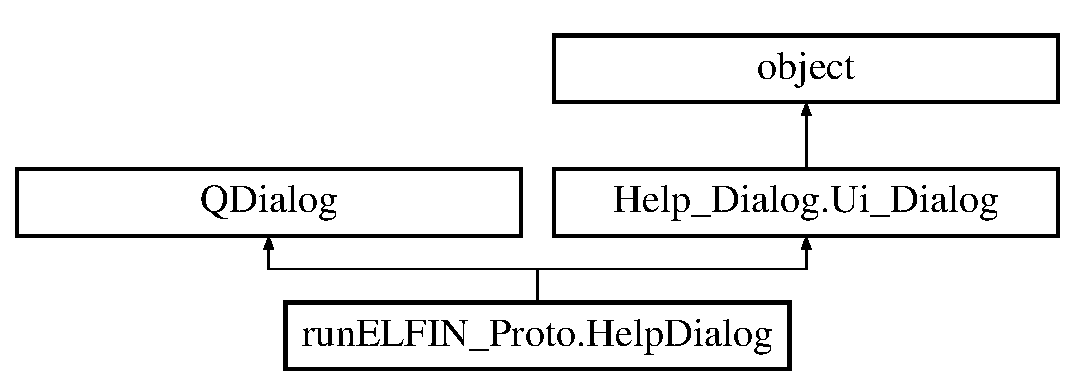
\includegraphics[height=3.000000cm]{classrunELFIN__Proto_1_1HelpDialog}
\end{center}
\end{figure}
\subsection*{Public Member Functions}
\begin{DoxyCompactItemize}
\item 
\hypertarget{classrunELFIN__Proto_1_1HelpDialog_af80d32e0edfb5fb4244a16220ba96de2}{def {\bfseries \-\_\-\-\_\-init\-\_\-\-\_\-}}\label{classrunELFIN__Proto_1_1HelpDialog_af80d32e0edfb5fb4244a16220ba96de2}

\item 
\hypertarget{classrunELFIN__Proto_1_1HelpDialog_a9bdb7b0d9ca12b76645a59ce8ad18a06}{def {\bfseries next\-\_\-page}}\label{classrunELFIN__Proto_1_1HelpDialog_a9bdb7b0d9ca12b76645a59ce8ad18a06}

\item 
\hypertarget{classrunELFIN__Proto_1_1HelpDialog_ac62d4e4a3483b9580038506b086e3561}{def {\bfseries prev\-\_\-page}}\label{classrunELFIN__Proto_1_1HelpDialog_ac62d4e4a3483b9580038506b086e3561}

\item 
\hypertarget{classrunELFIN__Proto_1_1HelpDialog_a4af56d945a598a2a03aa8a6de494d87b}{def {\bfseries close}}\label{classrunELFIN__Proto_1_1HelpDialog_a4af56d945a598a2a03aa8a6de494d87b}

\end{DoxyCompactItemize}
\subsection*{Public Attributes}
\begin{DoxyCompactItemize}
\item 
\hypertarget{classrunELFIN__Proto_1_1HelpDialog_a51a912a78cbd4e7d2246873f4b15974f}{{\bfseries total\-\_\-pages}}\label{classrunELFIN__Proto_1_1HelpDialog_a51a912a78cbd4e7d2246873f4b15974f}

\item 
\hypertarget{classrunELFIN__Proto_1_1HelpDialog_aca88e773346b803b15fc06f179bbbe12}{{\bfseries help\-\_\-done\-\_\-code}}\label{classrunELFIN__Proto_1_1HelpDialog_aca88e773346b803b15fc06f179bbbe12}

\end{DoxyCompactItemize}


The documentation for this class was generated from the following file\-:\begin{DoxyCompactItemize}
\item 
run\-E\-L\-F\-I\-N\-\_\-\-Proto.\-py\end{DoxyCompactItemize}

\hypertarget{classrunELFIN__Proto_1_1MyMainWindow}{\section{run\-E\-L\-F\-I\-N\-\_\-\-Proto.\-My\-Main\-Window Class Reference}
\label{classrunELFIN__Proto_1_1MyMainWindow}\index{run\-E\-L\-F\-I\-N\-\_\-\-Proto.\-My\-Main\-Window@{run\-E\-L\-F\-I\-N\-\_\-\-Proto.\-My\-Main\-Window}}
}


Main window for program.  


Inheritance diagram for run\-E\-L\-F\-I\-N\-\_\-\-Proto.\-My\-Main\-Window\-:\begin{figure}[H]
\begin{center}
\leavevmode
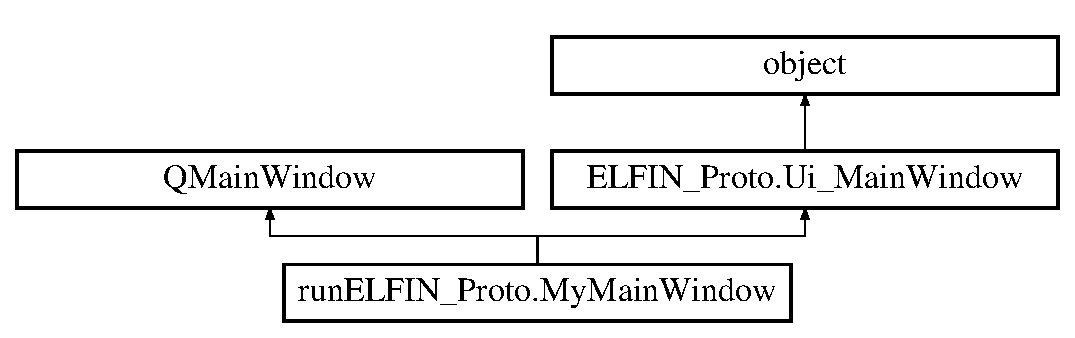
\includegraphics[height=3.000000cm]{classrunELFIN__Proto_1_1MyMainWindow}
\end{center}
\end{figure}
\subsection*{Public Member Functions}
\begin{DoxyCompactItemize}
\item 
\hypertarget{classrunELFIN__Proto_1_1MyMainWindow_ae712f1531c068f6a48c7995d24eedb8b}{def {\bfseries \-\_\-\-\_\-init\-\_\-\-\_\-}}\label{classrunELFIN__Proto_1_1MyMainWindow_ae712f1531c068f6a48c7995d24eedb8b}

\item 
\hypertarget{classrunELFIN__Proto_1_1MyMainWindow_a9b4d571c6951792edf26a520921001bb}{def {\bfseries display\-\_\-help\-\_\-dialog}}\label{classrunELFIN__Proto_1_1MyMainWindow_a9b4d571c6951792edf26a520921001bb}

\item 
\hypertarget{classrunELFIN__Proto_1_1MyMainWindow_a47b0dcac1776188a9e28056635fd7588}{def {\bfseries display\-\_\-add\-\_\-activity\-\_\-dialog}}\label{classrunELFIN__Proto_1_1MyMainWindow_a47b0dcac1776188a9e28056635fd7588}

\item 
\hypertarget{classrunELFIN__Proto_1_1MyMainWindow_aba72f11babfa66d80c11a046c09332d1}{def {\bfseries make\-\_\-draggable}}\label{classrunELFIN__Proto_1_1MyMainWindow_aba72f11babfa66d80c11a046c09332d1}

\item 
\hypertarget{classrunELFIN__Proto_1_1MyMainWindow_a525386f6f6547235982a0f20a3f0848c}{def {\bfseries turn\-\_\-on\-\_\-drag}}\label{classrunELFIN__Proto_1_1MyMainWindow_a525386f6f6547235982a0f20a3f0848c}

\item 
\hypertarget{classrunELFIN__Proto_1_1MyMainWindow_acaf9b8a013f9ea24f7256b33394997a4}{def {\bfseries turn\-\_\-off\-\_\-drag}}\label{classrunELFIN__Proto_1_1MyMainWindow_acaf9b8a013f9ea24f7256b33394997a4}

\item 
\hypertarget{classrunELFIN__Proto_1_1MyMainWindow_afb328c99232062f43609a3ad9adbd8b5}{def {\bfseries update\-\_\-item\-\_\-position}}\label{classrunELFIN__Proto_1_1MyMainWindow_afb328c99232062f43609a3ad9adbd8b5}

\end{DoxyCompactItemize}
\subsection*{Public Attributes}
\begin{DoxyCompactItemize}
\item 
\hypertarget{classrunELFIN__Proto_1_1MyMainWindow_a45e7c63b1e0cbe5cee870efa69b1f983}{{\bfseries scheduler}}\label{classrunELFIN__Proto_1_1MyMainWindow_a45e7c63b1e0cbe5cee870efa69b1f983}

\item 
\hypertarget{classrunELFIN__Proto_1_1MyMainWindow_a5ecf9793b56752f03a542b4ade9a7827}{{\bfseries drag\-\_\-timer}}\label{classrunELFIN__Proto_1_1MyMainWindow_a5ecf9793b56752f03a542b4ade9a7827}

\item 
\hypertarget{classrunELFIN__Proto_1_1MyMainWindow_a20694434bff9a7129222d3319e40cf9e}{{\bfseries drag\-\_\-wait\-\_\-interval}}\label{classrunELFIN__Proto_1_1MyMainWindow_a20694434bff9a7129222d3319e40cf9e}

\end{DoxyCompactItemize}


\subsection{Detailed Description}
Main window for program. 

The documentation for this class was generated from the following file\-:\begin{DoxyCompactItemize}
\item 
run\-E\-L\-F\-I\-N\-\_\-\-Proto.\-py\end{DoxyCompactItemize}

\hypertarget{classConsoleIO_1_1Override__Dialog}{\section{Console\-I\-O.\-Override\-\_\-\-Dialog Class Reference}
\label{classConsoleIO_1_1Override__Dialog}\index{Console\-I\-O.\-Override\-\_\-\-Dialog@{Console\-I\-O.\-Override\-\_\-\-Dialog}}
}


Requests and handles user input when a constraint violation can be overridden.  


Inheritance diagram for Console\-I\-O.\-Override\-\_\-\-Dialog\-:\begin{figure}[H]
\begin{center}
\leavevmode
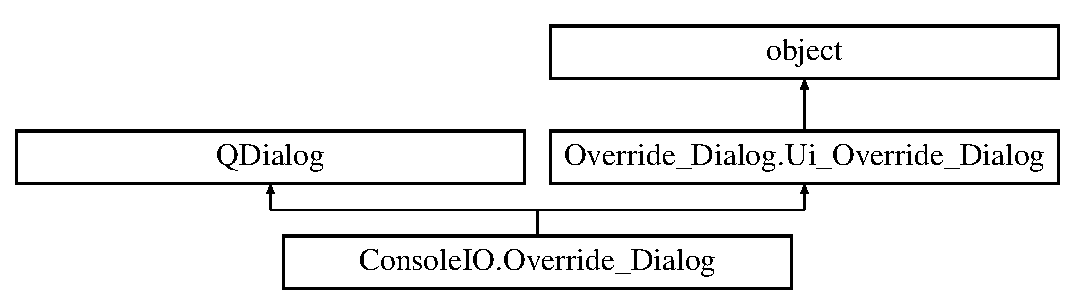
\includegraphics[height=3.000000cm]{classConsoleIO_1_1Override__Dialog}
\end{center}
\end{figure}
\subsection*{Public Member Functions}
\begin{DoxyCompactItemize}
\item 
\hypertarget{classConsoleIO_1_1Override__Dialog_aa15cd0546885e3d9943018d155a7538f}{def {\bfseries \-\_\-\-\_\-init\-\_\-\-\_\-}}\label{classConsoleIO_1_1Override__Dialog_aa15cd0546885e3d9943018d155a7538f}

\item 
\hypertarget{classConsoleIO_1_1Override__Dialog_a6afe1bfec98f696850eae66a89a9b312}{def {\bfseries yes\-\_\-input}}\label{classConsoleIO_1_1Override__Dialog_a6afe1bfec98f696850eae66a89a9b312}

\item 
\hypertarget{classConsoleIO_1_1Override__Dialog_a5c5aa5c0030a6820a900f3217309a91c}{def {\bfseries no\-\_\-input}}\label{classConsoleIO_1_1Override__Dialog_a5c5aa5c0030a6820a900f3217309a91c}

\item 
\hypertarget{classConsoleIO_1_1Override__Dialog_aeefa5a9c5257908082b0b636cd1692bb}{def {\bfseries close}}\label{classConsoleIO_1_1Override__Dialog_aeefa5a9c5257908082b0b636cd1692bb}

\end{DoxyCompactItemize}
\subsection*{Public Attributes}
\begin{DoxyCompactItemize}
\item 
\hypertarget{classConsoleIO_1_1Override__Dialog_a1a0207cdd4dd354bcf0d382b6e2f0ab9}{{\bfseries override\-\_\-done\-\_\-code}}\label{classConsoleIO_1_1Override__Dialog_a1a0207cdd4dd354bcf0d382b6e2f0ab9}

\end{DoxyCompactItemize}


\subsection{Detailed Description}
Requests and handles user input when a constraint violation can be overridden. 

The documentation for this class was generated from the following file\-:\begin{DoxyCompactItemize}
\item 
Console\-I\-O.\-py\end{DoxyCompactItemize}

\hypertarget{classScheduler_1_1Scheduler}{\section{Scheduler.\-Scheduler Class Reference}
\label{classScheduler_1_1Scheduler}\index{Scheduler.\-Scheduler@{Scheduler.\-Scheduler}}
}
\subsection*{Public Member Functions}
\begin{DoxyCompactItemize}
\item 
\hypertarget{classScheduler_1_1Scheduler_a4fe53057fd9abcf7be5accf58d8d8581}{def {\bfseries \-\_\-\-\_\-init\-\_\-\-\_\-}}\label{classScheduler_1_1Scheduler_a4fe53057fd9abcf7be5accf58d8d8581}

\item 
\hypertarget{classScheduler_1_1Scheduler_a564dfa584d5369be1bb95263fdf01227}{def {\bfseries add\-Activity}}\label{classScheduler_1_1Scheduler_a564dfa584d5369be1bb95263fdf01227}

\end{DoxyCompactItemize}
\subsection*{Public Attributes}
\begin{DoxyCompactItemize}
\item 
\hypertarget{classScheduler_1_1Scheduler_a3195eae6797c4d4fbdda1c70d7fbdde5}{{\bfseries qt\-Main\-Window}}\label{classScheduler_1_1Scheduler_a3195eae6797c4d4fbdda1c70d7fbdde5}

\item 
\hypertarget{classScheduler_1_1Scheduler_afb572141c16b677dbd4665907c59fc25}{{\bfseries console}}\label{classScheduler_1_1Scheduler_afb572141c16b677dbd4665907c59fc25}

\item 
\hypertarget{classScheduler_1_1Scheduler_a386637a091ac39683ba009a19be08b80}{{\bfseries database}}\label{classScheduler_1_1Scheduler_a386637a091ac39683ba009a19be08b80}

\item 
\hypertarget{classScheduler_1_1Scheduler_a4406548dfef2709fd5803c7fc9daa8ac}{{\bfseries constraints}}\label{classScheduler_1_1Scheduler_a4406548dfef2709fd5803c7fc9daa8ac}

\end{DoxyCompactItemize}


The documentation for this class was generated from the following file\-:\begin{DoxyCompactItemize}
\item 
Scheduler.\-py\end{DoxyCompactItemize}

\hypertarget{classAdd__Activity__Dialog_1_1Ui__Add__Activity__Dialog}{\section{Add\-\_\-\-Activity\-\_\-\-Dialog.\-Ui\-\_\-\-Add\-\_\-\-Activity\-\_\-\-Dialog Class Reference}
\label{classAdd__Activity__Dialog_1_1Ui__Add__Activity__Dialog}\index{Add\-\_\-\-Activity\-\_\-\-Dialog.\-Ui\-\_\-\-Add\-\_\-\-Activity\-\_\-\-Dialog@{Add\-\_\-\-Activity\-\_\-\-Dialog.\-Ui\-\_\-\-Add\-\_\-\-Activity\-\_\-\-Dialog}}
}
Inheritance diagram for Add\-\_\-\-Activity\-\_\-\-Dialog.\-Ui\-\_\-\-Add\-\_\-\-Activity\-\_\-\-Dialog\-:\begin{figure}[H]
\begin{center}
\leavevmode
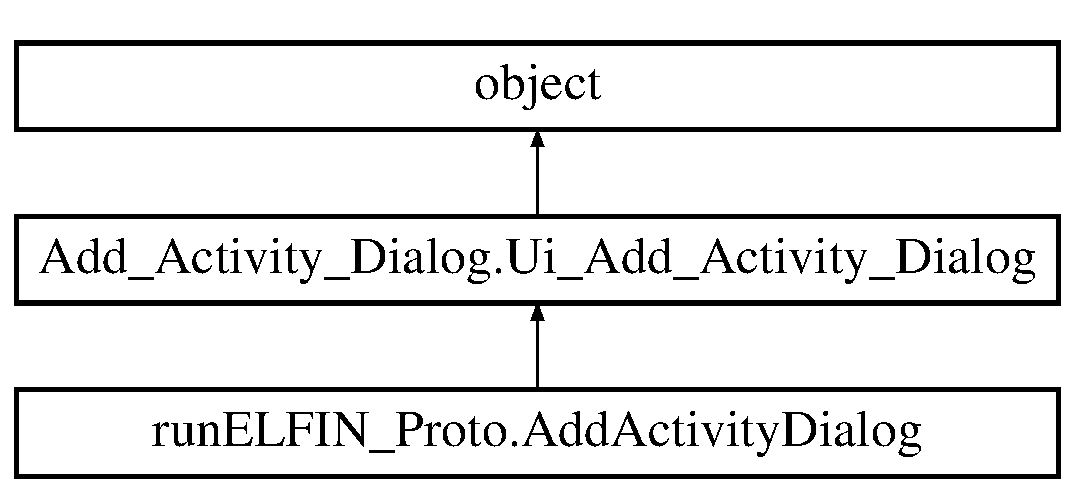
\includegraphics[height=3.000000cm]{classAdd__Activity__Dialog_1_1Ui__Add__Activity__Dialog}
\end{center}
\end{figure}
\subsection*{Public Member Functions}
\begin{DoxyCompactItemize}
\item 
\hypertarget{classAdd__Activity__Dialog_1_1Ui__Add__Activity__Dialog_acf37b8ba953fdc38c6f89f26ce922c61}{def {\bfseries setup\-Ui}}\label{classAdd__Activity__Dialog_1_1Ui__Add__Activity__Dialog_acf37b8ba953fdc38c6f89f26ce922c61}

\item 
\hypertarget{classAdd__Activity__Dialog_1_1Ui__Add__Activity__Dialog_a36b86b6a17f2dfce4268303d18cd22c1}{def {\bfseries retranslate\-Ui}}\label{classAdd__Activity__Dialog_1_1Ui__Add__Activity__Dialog_a36b86b6a17f2dfce4268303d18cd22c1}

\end{DoxyCompactItemize}
\subsection*{Public Attributes}
\begin{DoxyCompactItemize}
\item 
\hypertarget{classAdd__Activity__Dialog_1_1Ui__Add__Activity__Dialog_a6c8bfbc9319daf92c8cb0e1f958f2784}{{\bfseries parameters\-\_\-line\-\_\-edit}}\label{classAdd__Activity__Dialog_1_1Ui__Add__Activity__Dialog_a6c8bfbc9319daf92c8cb0e1f958f2784}

\item 
\hypertarget{classAdd__Activity__Dialog_1_1Ui__Add__Activity__Dialog_a50da5686c81904955e079a8578f7456b}{{\bfseries start\-\_\-time\-\_\-spin\-\_\-box}}\label{classAdd__Activity__Dialog_1_1Ui__Add__Activity__Dialog_a50da5686c81904955e079a8578f7456b}

\item 
\hypertarget{classAdd__Activity__Dialog_1_1Ui__Add__Activity__Dialog_a238137cdc487142424dd4d82d417b6b8}{{\bfseries stop\-\_\-time\-\_\-spin\-\_\-box}}\label{classAdd__Activity__Dialog_1_1Ui__Add__Activity__Dialog_a238137cdc487142424dd4d82d417b6b8}

\item 
\hypertarget{classAdd__Activity__Dialog_1_1Ui__Add__Activity__Dialog_aac73c5c79e58dbf3aa977cf7bd3560a3}{{\bfseries start\-\_\-time\-\_\-label}}\label{classAdd__Activity__Dialog_1_1Ui__Add__Activity__Dialog_aac73c5c79e58dbf3aa977cf7bd3560a3}

\item 
\hypertarget{classAdd__Activity__Dialog_1_1Ui__Add__Activity__Dialog_ae1bd08797f0bce8880fa8a288caca895}{{\bfseries stop\-\_\-time\-\_\-label}}\label{classAdd__Activity__Dialog_1_1Ui__Add__Activity__Dialog_ae1bd08797f0bce8880fa8a288caca895}

\item 
\hypertarget{classAdd__Activity__Dialog_1_1Ui__Add__Activity__Dialog_adeb794660ac76259c73fafdf0cec622a}{{\bfseries parameters\-\_\-label}}\label{classAdd__Activity__Dialog_1_1Ui__Add__Activity__Dialog_adeb794660ac76259c73fafdf0cec622a}

\item 
\hypertarget{classAdd__Activity__Dialog_1_1Ui__Add__Activity__Dialog_a825fda06f76e4320e6d6e3e41c7ffc2f}{{\bfseries main\-\_\-activity\-\_\-dialog\-\_\-label}}\label{classAdd__Activity__Dialog_1_1Ui__Add__Activity__Dialog_a825fda06f76e4320e6d6e3e41c7ffc2f}

\item 
\hypertarget{classAdd__Activity__Dialog_1_1Ui__Add__Activity__Dialog_a15cb7c40d9fb41a5b1f7f51d65ad0306}{{\bfseries activity\-\_\-view\-\_\-constraints\-\_\-button}}\label{classAdd__Activity__Dialog_1_1Ui__Add__Activity__Dialog_a15cb7c40d9fb41a5b1f7f51d65ad0306}

\item 
\hypertarget{classAdd__Activity__Dialog_1_1Ui__Add__Activity__Dialog_aedcfb85907502877643a1fc5e0aa0c86}{{\bfseries close\-\_\-button}}\label{classAdd__Activity__Dialog_1_1Ui__Add__Activity__Dialog_aedcfb85907502877643a1fc5e0aa0c86}

\item 
\hypertarget{classAdd__Activity__Dialog_1_1Ui__Add__Activity__Dialog_a20737594a903f5a6408906acdf606aca}{{\bfseries add\-\_\-activity\-\_\-button}}\label{classAdd__Activity__Dialog_1_1Ui__Add__Activity__Dialog_a20737594a903f5a6408906acdf606aca}

\item 
\hypertarget{classAdd__Activity__Dialog_1_1Ui__Add__Activity__Dialog_ab4b9edc3fbf12f78e73d45cc50647d1f}{{\bfseries thing\-\_\-label}}\label{classAdd__Activity__Dialog_1_1Ui__Add__Activity__Dialog_ab4b9edc3fbf12f78e73d45cc50647d1f}

\item 
\hypertarget{classAdd__Activity__Dialog_1_1Ui__Add__Activity__Dialog_aa3b9428365c11d3ad94cea9afb1615d9}{{\bfseries thing\-\_\-combo\-\_\-box}}\label{classAdd__Activity__Dialog_1_1Ui__Add__Activity__Dialog_aa3b9428365c11d3ad94cea9afb1615d9}

\end{DoxyCompactItemize}


The documentation for this class was generated from the following file\-:\begin{DoxyCompactItemize}
\item 
Add\-\_\-\-Activity\-\_\-\-Dialog.\-py\end{DoxyCompactItemize}

\hypertarget{classHelp__Dialog_1_1Ui__Dialog}{\section{Help\-\_\-\-Dialog.\-Ui\-\_\-\-Dialog Class Reference}
\label{classHelp__Dialog_1_1Ui__Dialog}\index{Help\-\_\-\-Dialog.\-Ui\-\_\-\-Dialog@{Help\-\_\-\-Dialog.\-Ui\-\_\-\-Dialog}}
}
Inheritance diagram for Help\-\_\-\-Dialog.\-Ui\-\_\-\-Dialog\-:\begin{figure}[H]
\begin{center}
\leavevmode
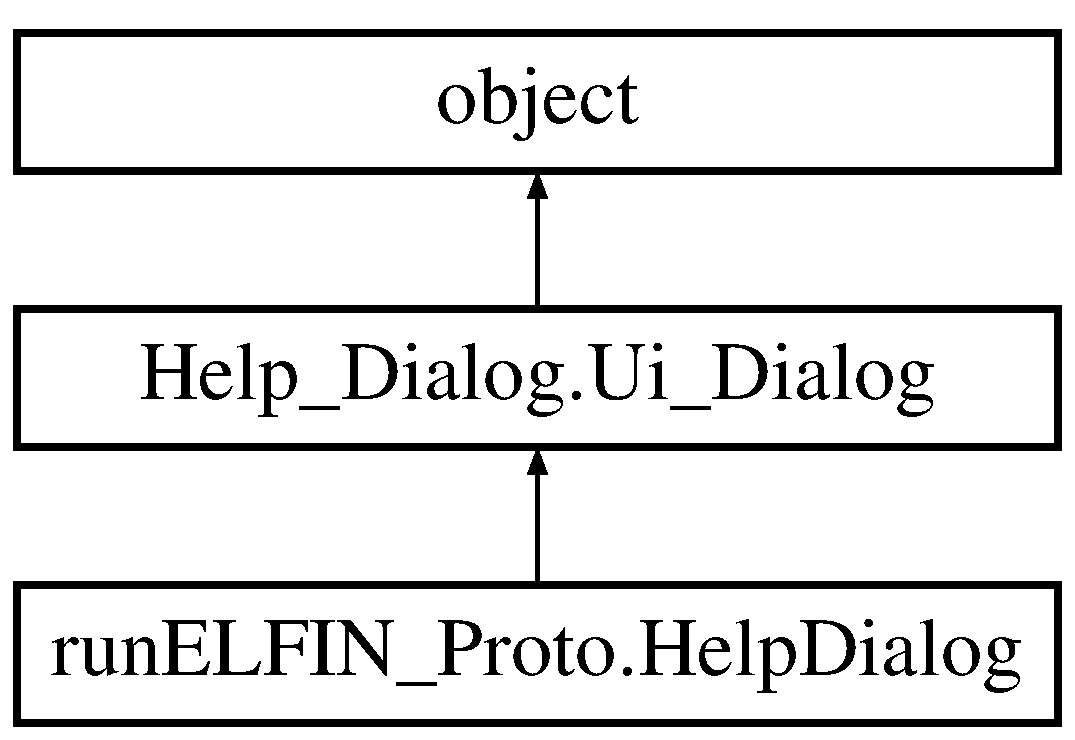
\includegraphics[height=3.000000cm]{classHelp__Dialog_1_1Ui__Dialog}
\end{center}
\end{figure}
\subsection*{Public Member Functions}
\begin{DoxyCompactItemize}
\item 
\hypertarget{classHelp__Dialog_1_1Ui__Dialog_af5886b2e0ede899c371ef0326bffa1ab}{def {\bfseries setup\-Ui}}\label{classHelp__Dialog_1_1Ui__Dialog_af5886b2e0ede899c371ef0326bffa1ab}

\item 
\hypertarget{classHelp__Dialog_1_1Ui__Dialog_a260cc059168a2f6e9e3d452c14d9b592}{def {\bfseries retranslate\-Ui}}\label{classHelp__Dialog_1_1Ui__Dialog_a260cc059168a2f6e9e3d452c14d9b592}

\end{DoxyCompactItemize}
\subsection*{Public Attributes}
\begin{DoxyCompactItemize}
\item 
\hypertarget{classHelp__Dialog_1_1Ui__Dialog_ab85265c2e22aa01bca5b0ea2eb3fd5b8}{{\bfseries help\-\_\-stacked\-Widget}}\label{classHelp__Dialog_1_1Ui__Dialog_ab85265c2e22aa01bca5b0ea2eb3fd5b8}

\item 
\hypertarget{classHelp__Dialog_1_1Ui__Dialog_a5c89ad437a02671441eeb1961ab41198}{{\bfseries page}}\label{classHelp__Dialog_1_1Ui__Dialog_a5c89ad437a02671441eeb1961ab41198}

\item 
\hypertarget{classHelp__Dialog_1_1Ui__Dialog_a74210b013a1e09d90e7bb7abcf464992}{{\bfseries schedule\-\_\-creator\-\_\-help\-\_\-label}}\label{classHelp__Dialog_1_1Ui__Dialog_a74210b013a1e09d90e7bb7abcf464992}

\item 
\hypertarget{classHelp__Dialog_1_1Ui__Dialog_a60677a16fcd018a0a8d5c2d605a0fa0a}{{\bfseries schedule\-\_\-creator\-\_\-help\-\_\-text\-\_\-edit}}\label{classHelp__Dialog_1_1Ui__Dialog_a60677a16fcd018a0a8d5c2d605a0fa0a}

\item 
\hypertarget{classHelp__Dialog_1_1Ui__Dialog_ac30ff6a87dd70aa0d9e8acac9d563af0}{{\bfseries page\-\_\-2}}\label{classHelp__Dialog_1_1Ui__Dialog_ac30ff6a87dd70aa0d9e8acac9d563af0}

\item 
\hypertarget{classHelp__Dialog_1_1Ui__Dialog_a0ebf41b7cceeeb679a7435644dd21d60}{{\bfseries schedule\-\_\-viewer\-\_\-help\-\_\-label}}\label{classHelp__Dialog_1_1Ui__Dialog_a0ebf41b7cceeeb679a7435644dd21d60}

\item 
\hypertarget{classHelp__Dialog_1_1Ui__Dialog_a099f0d3b41e06a5cdc1628ff90c54d5f}{{\bfseries schedule\-\_\-viewer\-\_\-help\-\_\-text\-\_\-edit}}\label{classHelp__Dialog_1_1Ui__Dialog_a099f0d3b41e06a5cdc1628ff90c54d5f}

\item 
\hypertarget{classHelp__Dialog_1_1Ui__Dialog_acc74151a4537de8da78ee5daf7f27bc2}{{\bfseries page\-\_\-3}}\label{classHelp__Dialog_1_1Ui__Dialog_acc74151a4537de8da78ee5daf7f27bc2}

\item 
\hypertarget{classHelp__Dialog_1_1Ui__Dialog_a413d83893970e81a8e10fe54f5f3bca4}{{\bfseries console\-\_\-help\-\_\-label\-\_\-2}}\label{classHelp__Dialog_1_1Ui__Dialog_a413d83893970e81a8e10fe54f5f3bca4}

\item 
\hypertarget{classHelp__Dialog_1_1Ui__Dialog_a61f485a9a6428e4ff27f4ddf2a782575}{{\bfseries console\-\_\-help\-\_\-text\-\_\-edit}}\label{classHelp__Dialog_1_1Ui__Dialog_a61f485a9a6428e4ff27f4ddf2a782575}

\item 
\hypertarget{classHelp__Dialog_1_1Ui__Dialog_ad1c79d0b8660d10bcd5525f7033e9b4e}{{\bfseries help\-\_\-done\-\_\-button}}\label{classHelp__Dialog_1_1Ui__Dialog_ad1c79d0b8660d10bcd5525f7033e9b4e}

\item 
\hypertarget{classHelp__Dialog_1_1Ui__Dialog_ad6b493cc7614d98c197ece6fe674f52b}{{\bfseries help\-\_\-next\-\_\-button}}\label{classHelp__Dialog_1_1Ui__Dialog_ad6b493cc7614d98c197ece6fe674f52b}

\item 
\hypertarget{classHelp__Dialog_1_1Ui__Dialog_a93638041308b0613939e1d2e3b4b13b8}{{\bfseries help\-\_\-prev\-\_\-button}}\label{classHelp__Dialog_1_1Ui__Dialog_a93638041308b0613939e1d2e3b4b13b8}

\end{DoxyCompactItemize}


The documentation for this class was generated from the following file\-:\begin{DoxyCompactItemize}
\item 
Help\-\_\-\-Dialog.\-py\end{DoxyCompactItemize}

\hypertarget{classELFIN__Proto_1_1Ui__MainWindow}{\section{E\-L\-F\-I\-N\-\_\-\-Proto.\-Ui\-\_\-\-Main\-Window Class Reference}
\label{classELFIN__Proto_1_1Ui__MainWindow}\index{E\-L\-F\-I\-N\-\_\-\-Proto.\-Ui\-\_\-\-Main\-Window@{E\-L\-F\-I\-N\-\_\-\-Proto.\-Ui\-\_\-\-Main\-Window}}
}
Inheritance diagram for E\-L\-F\-I\-N\-\_\-\-Proto.\-Ui\-\_\-\-Main\-Window\-:\begin{figure}[H]
\begin{center}
\leavevmode
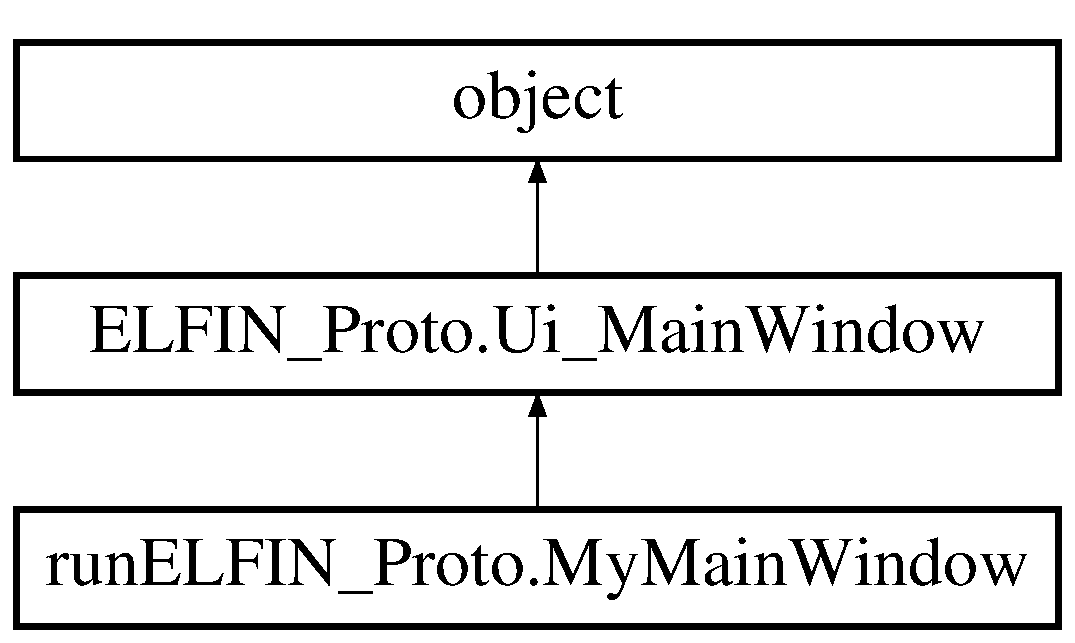
\includegraphics[height=3.000000cm]{classELFIN__Proto_1_1Ui__MainWindow}
\end{center}
\end{figure}
\subsection*{Public Member Functions}
\begin{DoxyCompactItemize}
\item 
\hypertarget{classELFIN__Proto_1_1Ui__MainWindow_a79285f206f571c8615ca10984de1ec34}{def {\bfseries setup\-Ui}}\label{classELFIN__Proto_1_1Ui__MainWindow_a79285f206f571c8615ca10984de1ec34}

\item 
\hypertarget{classELFIN__Proto_1_1Ui__MainWindow_a440ebc99241b0411d44d305985e27048}{def {\bfseries retranslate\-Ui}}\label{classELFIN__Proto_1_1Ui__MainWindow_a440ebc99241b0411d44d305985e27048}

\end{DoxyCompactItemize}
\subsection*{Public Attributes}
\begin{DoxyCompactItemize}
\item 
\hypertarget{classELFIN__Proto_1_1Ui__MainWindow_a5c15b17f3957fde52e589bf646fe79a1}{{\bfseries centralwidget}}\label{classELFIN__Proto_1_1Ui__MainWindow_a5c15b17f3957fde52e589bf646fe79a1}

\item 
\hypertarget{classELFIN__Proto_1_1Ui__MainWindow_aadf7b908fdadf81c72b758be54a810e6}{{\bfseries tab\-Control}}\label{classELFIN__Proto_1_1Ui__MainWindow_aadf7b908fdadf81c72b758be54a810e6}

\item 
\hypertarget{classELFIN__Proto_1_1Ui__MainWindow_ac373b7e53e2dc1d6aba7bc71d443a66b}{{\bfseries tab}}\label{classELFIN__Proto_1_1Ui__MainWindow_ac373b7e53e2dc1d6aba7bc71d443a66b}

\item 
\hypertarget{classELFIN__Proto_1_1Ui__MainWindow_a59d432966dded7539e5a193b7a98fba6}{{\bfseries schedule\-\_\-viewer\-\_\-group\-\_\-box}}\label{classELFIN__Proto_1_1Ui__MainWindow_a59d432966dded7539e5a193b7a98fba6}

\item 
\hypertarget{classELFIN__Proto_1_1Ui__MainWindow_a2506466a1a251fd72b4c5c000ce0d47f}{{\bfseries label}}\label{classELFIN__Proto_1_1Ui__MainWindow_a2506466a1a251fd72b4c5c000ce0d47f}

\item 
\hypertarget{classELFIN__Proto_1_1Ui__MainWindow_add74a0c8c15eb59c64e81717795f6d2d}{{\bfseries label\-\_\-2}}\label{classELFIN__Proto_1_1Ui__MainWindow_add74a0c8c15eb59c64e81717795f6d2d}

\item 
\hypertarget{classELFIN__Proto_1_1Ui__MainWindow_a170840d82323d03352eef276cff817bb}{{\bfseries label\-\_\-3}}\label{classELFIN__Proto_1_1Ui__MainWindow_a170840d82323d03352eef276cff817bb}

\item 
\hypertarget{classELFIN__Proto_1_1Ui__MainWindow_a9902d744649af259709518a80304847b}{{\bfseries label\-\_\-4}}\label{classELFIN__Proto_1_1Ui__MainWindow_a9902d744649af259709518a80304847b}

\item 
\hypertarget{classELFIN__Proto_1_1Ui__MainWindow_a08ee8cc52ac46529804063e302cb397f}{{\bfseries label\-\_\-5}}\label{classELFIN__Proto_1_1Ui__MainWindow_a08ee8cc52ac46529804063e302cb397f}

\item 
\hypertarget{classELFIN__Proto_1_1Ui__MainWindow_a2d0714caf42cec182949c998391b04d3}{{\bfseries schedule\-\_\-viewer\-\_\-label}}\label{classELFIN__Proto_1_1Ui__MainWindow_a2d0714caf42cec182949c998391b04d3}

\item 
\hypertarget{classELFIN__Proto_1_1Ui__MainWindow_aeb0452b33693adf737772e3590bceb39}{{\bfseries example\-\_\-zone\-\_\-2}}\label{classELFIN__Proto_1_1Ui__MainWindow_aeb0452b33693adf737772e3590bceb39}

\item 
\hypertarget{classELFIN__Proto_1_1Ui__MainWindow_a52b7f90b8b636d7d7966724b28ced952}{{\bfseries example\-\_\-event\-\_\-1}}\label{classELFIN__Proto_1_1Ui__MainWindow_a52b7f90b8b636d7d7966724b28ced952}

\item 
\hypertarget{classELFIN__Proto_1_1Ui__MainWindow_aff091beb966545431b6053d071275e96}{{\bfseries example\-\_\-zone\-\_\-1}}\label{classELFIN__Proto_1_1Ui__MainWindow_aff091beb966545431b6053d071275e96}

\item 
\hypertarget{classELFIN__Proto_1_1Ui__MainWindow_a00f1df79cf9d43ed7a56d8351329aa02}{{\bfseries horizontal\-\_\-line\-\_\-4}}\label{classELFIN__Proto_1_1Ui__MainWindow_a00f1df79cf9d43ed7a56d8351329aa02}

\item 
\hypertarget{classELFIN__Proto_1_1Ui__MainWindow_a7d0764bfaa17a30751c1742234dfdfec}{{\bfseries horizontal\-\_\-line\-\_\-1}}\label{classELFIN__Proto_1_1Ui__MainWindow_a7d0764bfaa17a30751c1742234dfdfec}

\item 
\hypertarget{classELFIN__Proto_1_1Ui__MainWindow_a6abe873b7e63db1b6f217ed6216a1f27}{{\bfseries horizontal\-\_\-line\-\_\-5}}\label{classELFIN__Proto_1_1Ui__MainWindow_a6abe873b7e63db1b6f217ed6216a1f27}

\item 
\hypertarget{classELFIN__Proto_1_1Ui__MainWindow_a1d84a8ec80bda58ff49e6d6150dcc683}{{\bfseries horizontal\-\_\-line\-\_\-3}}\label{classELFIN__Proto_1_1Ui__MainWindow_a1d84a8ec80bda58ff49e6d6150dcc683}

\item 
\hypertarget{classELFIN__Proto_1_1Ui__MainWindow_a200d2186edf52cc9fe6a2abbd23ba3ef}{{\bfseries horizontal\-\_\-line\-\_\-2}}\label{classELFIN__Proto_1_1Ui__MainWindow_a200d2186edf52cc9fe6a2abbd23ba3ef}

\item 
\hypertarget{classELFIN__Proto_1_1Ui__MainWindow_a9a740c7ac8f2cba0ad74dee4654075ac}{{\bfseries example\-\_\-time\-\_\-label\-\_\-1}}\label{classELFIN__Proto_1_1Ui__MainWindow_a9a740c7ac8f2cba0ad74dee4654075ac}

\item 
\hypertarget{classELFIN__Proto_1_1Ui__MainWindow_adc6447ee1620fd1ea3fbd00bb12c1cca}{{\bfseries example\-\_\-time\-\_\-label\-\_\-2}}\label{classELFIN__Proto_1_1Ui__MainWindow_adc6447ee1620fd1ea3fbd00bb12c1cca}

\item 
\hypertarget{classELFIN__Proto_1_1Ui__MainWindow_a825619be0f85a51b1cd72b93416a3a4e}{{\bfseries example\-\_\-time\-\_\-label\-\_\-3}}\label{classELFIN__Proto_1_1Ui__MainWindow_a825619be0f85a51b1cd72b93416a3a4e}

\item 
\hypertarget{classELFIN__Proto_1_1Ui__MainWindow_a28b8834707b2f3d0fee52d6ce98209ca}{{\bfseries example\-\_\-time\-\_\-label\-\_\-4}}\label{classELFIN__Proto_1_1Ui__MainWindow_a28b8834707b2f3d0fee52d6ce98209ca}

\item 
\hypertarget{classELFIN__Proto_1_1Ui__MainWindow_a3fff18209eeb2b59691e4933ae4fd950}{{\bfseries example\-\_\-time\-\_\-label\-\_\-5}}\label{classELFIN__Proto_1_1Ui__MainWindow_a3fff18209eeb2b59691e4933ae4fd950}

\item 
\hypertarget{classELFIN__Proto_1_1Ui__MainWindow_a8135181cc7c078a3106ab5ead9052d3d}{{\bfseries example\-\_\-time\-\_\-label\-\_\-6}}\label{classELFIN__Proto_1_1Ui__MainWindow_a8135181cc7c078a3106ab5ead9052d3d}

\item 
\hypertarget{classELFIN__Proto_1_1Ui__MainWindow_a1bd9f1f9dce194b2516766a3a9304078}{{\bfseries example\-\_\-time\-\_\-label\-\_\-7}}\label{classELFIN__Proto_1_1Ui__MainWindow_a1bd9f1f9dce194b2516766a3a9304078}

\item 
\hypertarget{classELFIN__Proto_1_1Ui__MainWindow_a91dbfdca2f704c2da17af16a94ac849a}{{\bfseries example\-\_\-time\-\_\-label\-\_\-8}}\label{classELFIN__Proto_1_1Ui__MainWindow_a91dbfdca2f704c2da17af16a94ac849a}

\item 
\hypertarget{classELFIN__Proto_1_1Ui__MainWindow_a22baacf261b3cbe7d1486a21fba72de7}{{\bfseries example\-\_\-time\-\_\-label\-\_\-9}}\label{classELFIN__Proto_1_1Ui__MainWindow_a22baacf261b3cbe7d1486a21fba72de7}

\item 
\hypertarget{classELFIN__Proto_1_1Ui__MainWindow_a7f78e0037cef4425b317ea045e02b351}{{\bfseries example\-\_\-time\-\_\-label\-\_\-10}}\label{classELFIN__Proto_1_1Ui__MainWindow_a7f78e0037cef4425b317ea045e02b351}

\item 
\hypertarget{classELFIN__Proto_1_1Ui__MainWindow_a8983a0706fc9c918d894362bedb78b91}{{\bfseries vertical\-\_\-line\-\_\-1}}\label{classELFIN__Proto_1_1Ui__MainWindow_a8983a0706fc9c918d894362bedb78b91}

\item 
\hypertarget{classELFIN__Proto_1_1Ui__MainWindow_a94ec022ce2dcd55ea9815d16e01eab9e}{{\bfseries vertical\-\_\-line\-\_\-2}}\label{classELFIN__Proto_1_1Ui__MainWindow_a94ec022ce2dcd55ea9815d16e01eab9e}

\item 
\hypertarget{classELFIN__Proto_1_1Ui__MainWindow_a6b1772a9f7c1c42c7babf08426ea47d7}{{\bfseries vertical\-\_\-line\-\_\-3}}\label{classELFIN__Proto_1_1Ui__MainWindow_a6b1772a9f7c1c42c7babf08426ea47d7}

\item 
\hypertarget{classELFIN__Proto_1_1Ui__MainWindow_aa3de605db7d40a067305958b7529993a}{{\bfseries vertical\-\_\-line\-\_\-4}}\label{classELFIN__Proto_1_1Ui__MainWindow_aa3de605db7d40a067305958b7529993a}

\item 
\hypertarget{classELFIN__Proto_1_1Ui__MainWindow_a79c448dc7a0a46551e14f8559fa9186c}{{\bfseries vertical\-\_\-line\-\_\-5}}\label{classELFIN__Proto_1_1Ui__MainWindow_a79c448dc7a0a46551e14f8559fa9186c}

\item 
\hypertarget{classELFIN__Proto_1_1Ui__MainWindow_a3d29ce8e47d720cfb18a350aa7456bc1}{{\bfseries vertical\-\_\-line\-\_\-6}}\label{classELFIN__Proto_1_1Ui__MainWindow_a3d29ce8e47d720cfb18a350aa7456bc1}

\item 
\hypertarget{classELFIN__Proto_1_1Ui__MainWindow_a6cf4955bd758f405328f446be592cffa}{{\bfseries vertical\-\_\-line\-\_\-7}}\label{classELFIN__Proto_1_1Ui__MainWindow_a6cf4955bd758f405328f446be592cffa}

\item 
\hypertarget{classELFIN__Proto_1_1Ui__MainWindow_a5a30f063a317261af3d00b9069212be7}{{\bfseries vertical\-\_\-line\-\_\-8}}\label{classELFIN__Proto_1_1Ui__MainWindow_a5a30f063a317261af3d00b9069212be7}

\item 
\hypertarget{classELFIN__Proto_1_1Ui__MainWindow_a663baf89d453a49eca2e0a5f18c33122}{{\bfseries vertical\-\_\-line\-\_\-9}}\label{classELFIN__Proto_1_1Ui__MainWindow_a663baf89d453a49eca2e0a5f18c33122}

\item 
\hypertarget{classELFIN__Proto_1_1Ui__MainWindow_a1b6a79885c43b1103670405cb659ac83}{{\bfseries vertical\-\_\-line\-\_\-10}}\label{classELFIN__Proto_1_1Ui__MainWindow_a1b6a79885c43b1103670405cb659ac83}

\item 
\hypertarget{classELFIN__Proto_1_1Ui__MainWindow_a5121aeeff57565ba83647cef8fc31e8b}{{\bfseries example\-\_\-activity\-\_\-label\-\_\-1}}\label{classELFIN__Proto_1_1Ui__MainWindow_a5121aeeff57565ba83647cef8fc31e8b}

\item 
\hypertarget{classELFIN__Proto_1_1Ui__MainWindow_a1ac8ff73d327bce996feaaa6e2b2d1bf}{{\bfseries example\-\_\-activity\-\_\-label\-\_\-2}}\label{classELFIN__Proto_1_1Ui__MainWindow_a1ac8ff73d327bce996feaaa6e2b2d1bf}

\item 
\hypertarget{classELFIN__Proto_1_1Ui__MainWindow_aeb91e6566aa5e306badd83afe049aba8}{{\bfseries schedule\-\_\-viewer\-\_\-scroll\-\_\-bar}}\label{classELFIN__Proto_1_1Ui__MainWindow_aeb91e6566aa5e306badd83afe049aba8}

\item 
\hypertarget{classELFIN__Proto_1_1Ui__MainWindow_a3f273860527422b9526cb0df32629d18}{{\bfseries tab\-\_\-2}}\label{classELFIN__Proto_1_1Ui__MainWindow_a3f273860527422b9526cb0df32629d18}

\item 
\hypertarget{classELFIN__Proto_1_1Ui__MainWindow_ad56b19a9a99798a028f15e437ff26c85}{{\bfseries schedule\-\_\-creator\-\_\-group\-\_\-box}}\label{classELFIN__Proto_1_1Ui__MainWindow_ad56b19a9a99798a028f15e437ff26c85}

\item 
\hypertarget{classELFIN__Proto_1_1Ui__MainWindow_a7a4d5f86058cc1889b555ef09ba19f68}{{\bfseries label\-\_\-6}}\label{classELFIN__Proto_1_1Ui__MainWindow_a7a4d5f86058cc1889b555ef09ba19f68}

\item 
\hypertarget{classELFIN__Proto_1_1Ui__MainWindow_a92afd381cd97bc258a7395536242774f}{{\bfseries label\-\_\-7}}\label{classELFIN__Proto_1_1Ui__MainWindow_a92afd381cd97bc258a7395536242774f}

\item 
\hypertarget{classELFIN__Proto_1_1Ui__MainWindow_ad4c919c2c16198cfc97f79a75b6d0282}{{\bfseries label\-\_\-8}}\label{classELFIN__Proto_1_1Ui__MainWindow_ad4c919c2c16198cfc97f79a75b6d0282}

\item 
\hypertarget{classELFIN__Proto_1_1Ui__MainWindow_af79609f7a1058323cb6f01f179ea260c}{{\bfseries label\-\_\-9}}\label{classELFIN__Proto_1_1Ui__MainWindow_af79609f7a1058323cb6f01f179ea260c}

\item 
\hypertarget{classELFIN__Proto_1_1Ui__MainWindow_ac67915778c382baa7f69b5f68654a912}{{\bfseries label\-\_\-10}}\label{classELFIN__Proto_1_1Ui__MainWindow_ac67915778c382baa7f69b5f68654a912}

\item 
\hypertarget{classELFIN__Proto_1_1Ui__MainWindow_a49bf192e080762e4bfe1158a54800fb5}{{\bfseries schedule\-\_\-viewer\-\_\-label\-\_\-2}}\label{classELFIN__Proto_1_1Ui__MainWindow_a49bf192e080762e4bfe1158a54800fb5}

\item 
\hypertarget{classELFIN__Proto_1_1Ui__MainWindow_abd8cbd2256e4ff13e3f97ea5e7050a60}{{\bfseries example\-\_\-zone\-\_\-3}}\label{classELFIN__Proto_1_1Ui__MainWindow_abd8cbd2256e4ff13e3f97ea5e7050a60}

\item 
\hypertarget{classELFIN__Proto_1_1Ui__MainWindow_aafc53891c75088c0cab1a0756cfa9914}{{\bfseries example\-\_\-event\-\_\-2}}\label{classELFIN__Proto_1_1Ui__MainWindow_aafc53891c75088c0cab1a0756cfa9914}

\item 
\hypertarget{classELFIN__Proto_1_1Ui__MainWindow_aa6f5178db00bb511a148e528d9cd185a}{{\bfseries example\-\_\-zone\-\_\-4}}\label{classELFIN__Proto_1_1Ui__MainWindow_aa6f5178db00bb511a148e528d9cd185a}

\item 
\hypertarget{classELFIN__Proto_1_1Ui__MainWindow_a549c99f1bfd7a90d2c9fab88eafc2c61}{{\bfseries horizontal\-\_\-line\-\_\-6}}\label{classELFIN__Proto_1_1Ui__MainWindow_a549c99f1bfd7a90d2c9fab88eafc2c61}

\item 
\hypertarget{classELFIN__Proto_1_1Ui__MainWindow_a52a44d43eadf6ee2a108fee1a8de5c76}{{\bfseries horizontal\-\_\-line\-\_\-7}}\label{classELFIN__Proto_1_1Ui__MainWindow_a52a44d43eadf6ee2a108fee1a8de5c76}

\item 
\hypertarget{classELFIN__Proto_1_1Ui__MainWindow_aef29bf6880e1b4ae8edf47918c63a4e8}{{\bfseries horizontal\-\_\-line\-\_\-8}}\label{classELFIN__Proto_1_1Ui__MainWindow_aef29bf6880e1b4ae8edf47918c63a4e8}

\item 
\hypertarget{classELFIN__Proto_1_1Ui__MainWindow_a1e9a40f7035fa3df5596d941a405a788}{{\bfseries horizontal\-\_\-line\-\_\-9}}\label{classELFIN__Proto_1_1Ui__MainWindow_a1e9a40f7035fa3df5596d941a405a788}

\item 
\hypertarget{classELFIN__Proto_1_1Ui__MainWindow_a6af1da459a3690ba43c72ec458b0fde9}{{\bfseries horizontal\-\_\-line\-\_\-10}}\label{classELFIN__Proto_1_1Ui__MainWindow_a6af1da459a3690ba43c72ec458b0fde9}

\item 
\hypertarget{classELFIN__Proto_1_1Ui__MainWindow_ad69e5fa6a4fb177dd535874cd49a76f6}{{\bfseries example\-\_\-time\-\_\-label\-\_\-11}}\label{classELFIN__Proto_1_1Ui__MainWindow_ad69e5fa6a4fb177dd535874cd49a76f6}

\item 
\hypertarget{classELFIN__Proto_1_1Ui__MainWindow_a1521ce7de93a1a6ba57bf0547457fb70}{{\bfseries example\-\_\-time\-\_\-label\-\_\-12}}\label{classELFIN__Proto_1_1Ui__MainWindow_a1521ce7de93a1a6ba57bf0547457fb70}

\item 
\hypertarget{classELFIN__Proto_1_1Ui__MainWindow_a336b094d19190559899a993ed952dbc1}{{\bfseries example\-\_\-time\-\_\-label\-\_\-13}}\label{classELFIN__Proto_1_1Ui__MainWindow_a336b094d19190559899a993ed952dbc1}

\item 
\hypertarget{classELFIN__Proto_1_1Ui__MainWindow_a15b0d9ff63b96e483e4d01da817902e4}{{\bfseries example\-\_\-time\-\_\-label\-\_\-14}}\label{classELFIN__Proto_1_1Ui__MainWindow_a15b0d9ff63b96e483e4d01da817902e4}

\item 
\hypertarget{classELFIN__Proto_1_1Ui__MainWindow_af655fc659009b2b0bb5019acccf711a6}{{\bfseries example\-\_\-time\-\_\-label\-\_\-15}}\label{classELFIN__Proto_1_1Ui__MainWindow_af655fc659009b2b0bb5019acccf711a6}

\item 
\hypertarget{classELFIN__Proto_1_1Ui__MainWindow_a185abc569968dff86098f69d846613c1}{{\bfseries example\-\_\-time\-\_\-label\-\_\-16}}\label{classELFIN__Proto_1_1Ui__MainWindow_a185abc569968dff86098f69d846613c1}

\item 
\hypertarget{classELFIN__Proto_1_1Ui__MainWindow_aed0a45c9630155a49a90a9e6f6b63737}{{\bfseries example\-\_\-time\-\_\-label\-\_\-17}}\label{classELFIN__Proto_1_1Ui__MainWindow_aed0a45c9630155a49a90a9e6f6b63737}

\item 
\hypertarget{classELFIN__Proto_1_1Ui__MainWindow_a8160d2f3111acfe435ae72600bd0480f}{{\bfseries example\-\_\-time\-\_\-label\-\_\-18}}\label{classELFIN__Proto_1_1Ui__MainWindow_a8160d2f3111acfe435ae72600bd0480f}

\item 
\hypertarget{classELFIN__Proto_1_1Ui__MainWindow_a43832402b867c0bb1b6a01aad7e255e6}{{\bfseries example\-\_\-time\-\_\-label\-\_\-19}}\label{classELFIN__Proto_1_1Ui__MainWindow_a43832402b867c0bb1b6a01aad7e255e6}

\item 
\hypertarget{classELFIN__Proto_1_1Ui__MainWindow_ad314a8d84f3d1a5790ced50160663c38}{{\bfseries example\-\_\-time\-\_\-label\-\_\-20}}\label{classELFIN__Proto_1_1Ui__MainWindow_ad314a8d84f3d1a5790ced50160663c38}

\item 
\hypertarget{classELFIN__Proto_1_1Ui__MainWindow_aa68f60f0dd40f7ccddf54565c7c4c691}{{\bfseries vertical\-\_\-line\-\_\-11}}\label{classELFIN__Proto_1_1Ui__MainWindow_aa68f60f0dd40f7ccddf54565c7c4c691}

\item 
\hypertarget{classELFIN__Proto_1_1Ui__MainWindow_aa0709df70655e8d1413d260751ff0744}{{\bfseries vertical\-\_\-line\-\_\-12}}\label{classELFIN__Proto_1_1Ui__MainWindow_aa0709df70655e8d1413d260751ff0744}

\item 
\hypertarget{classELFIN__Proto_1_1Ui__MainWindow_a5b6bd07f88f2a4dc12b3b2c971ef36b5}{{\bfseries vertical\-\_\-line\-\_\-13}}\label{classELFIN__Proto_1_1Ui__MainWindow_a5b6bd07f88f2a4dc12b3b2c971ef36b5}

\item 
\hypertarget{classELFIN__Proto_1_1Ui__MainWindow_a66c4c2c12d989fd6c6aced5acb76601c}{{\bfseries vertical\-\_\-line\-\_\-14}}\label{classELFIN__Proto_1_1Ui__MainWindow_a66c4c2c12d989fd6c6aced5acb76601c}

\item 
\hypertarget{classELFIN__Proto_1_1Ui__MainWindow_ae145271f97798c22e8893128fc101f5f}{{\bfseries vertical\-\_\-line\-\_\-15}}\label{classELFIN__Proto_1_1Ui__MainWindow_ae145271f97798c22e8893128fc101f5f}

\item 
\hypertarget{classELFIN__Proto_1_1Ui__MainWindow_af62985ab892605fe4bea41fa5b86a508}{{\bfseries vertical\-\_\-line\-\_\-16}}\label{classELFIN__Proto_1_1Ui__MainWindow_af62985ab892605fe4bea41fa5b86a508}

\item 
\hypertarget{classELFIN__Proto_1_1Ui__MainWindow_a57eff8f27ff9319f99dbf29dc279b6fe}{{\bfseries vertical\-\_\-line\-\_\-17}}\label{classELFIN__Proto_1_1Ui__MainWindow_a57eff8f27ff9319f99dbf29dc279b6fe}

\item 
\hypertarget{classELFIN__Proto_1_1Ui__MainWindow_a0ba32a57c3dea48d6943498b7f7e47a7}{{\bfseries vertical\-\_\-line\-\_\-18}}\label{classELFIN__Proto_1_1Ui__MainWindow_a0ba32a57c3dea48d6943498b7f7e47a7}

\item 
\hypertarget{classELFIN__Proto_1_1Ui__MainWindow_a5137fc2e19dad44b3512ff06475bf6eb}{{\bfseries vertical\-\_\-line\-\_\-19}}\label{classELFIN__Proto_1_1Ui__MainWindow_a5137fc2e19dad44b3512ff06475bf6eb}

\item 
\hypertarget{classELFIN__Proto_1_1Ui__MainWindow_a585a4bd30b71dad574511c3c75525b52}{{\bfseries vertical\-\_\-line\-\_\-20}}\label{classELFIN__Proto_1_1Ui__MainWindow_a585a4bd30b71dad574511c3c75525b52}

\item 
\hypertarget{classELFIN__Proto_1_1Ui__MainWindow_a08cfbbc981b6b78f550ef57de23273b6}{{\bfseries add\-\_\-activity\-\_\-button}}\label{classELFIN__Proto_1_1Ui__MainWindow_a08cfbbc981b6b78f550ef57de23273b6}

\item 
\hypertarget{classELFIN__Proto_1_1Ui__MainWindow_a54eca1dc5aecceec2c6700b97961b837}{{\bfseries example\-\_\-activity\-\_\-button\-\_\-1}}\label{classELFIN__Proto_1_1Ui__MainWindow_a54eca1dc5aecceec2c6700b97961b837}

\item 
\hypertarget{classELFIN__Proto_1_1Ui__MainWindow_ac56d873f3ff2a7b8d589711ceefbd55c}{{\bfseries example\-\_\-activity\-\_\-button\-\_\-2}}\label{classELFIN__Proto_1_1Ui__MainWindow_ac56d873f3ff2a7b8d589711ceefbd55c}

\item 
\hypertarget{classELFIN__Proto_1_1Ui__MainWindow_a793b2f9d8588a234a8a0415f69e3a79e}{{\bfseries schedule\-\_\-viewer\-\_\-scroll\-\_\-bar\-\_\-2}}\label{classELFIN__Proto_1_1Ui__MainWindow_a793b2f9d8588a234a8a0415f69e3a79e}

\item 
\hypertarget{classELFIN__Proto_1_1Ui__MainWindow_acc260f21f0bca08ca3ba385ae8f94346}{{\bfseries tab\-\_\-5}}\label{classELFIN__Proto_1_1Ui__MainWindow_acc260f21f0bca08ca3ba385ae8f94346}

\item 
\hypertarget{classELFIN__Proto_1_1Ui__MainWindow_adfe3a5daac34b752d21cc5a912d788f4}{{\bfseries graphics\-\_\-scene\-\_\-test\-\_\-view}}\label{classELFIN__Proto_1_1Ui__MainWindow_adfe3a5daac34b752d21cc5a912d788f4}

\item 
\hypertarget{classELFIN__Proto_1_1Ui__MainWindow_a83feb92c61a859bbc07e0abf160d603f}{{\bfseries tab\-Widget\-\_\-2}}\label{classELFIN__Proto_1_1Ui__MainWindow_a83feb92c61a859bbc07e0abf160d603f}

\item 
\hypertarget{classELFIN__Proto_1_1Ui__MainWindow_a3d7e317b4e2dadbd7fef47aafbde8461}{{\bfseries tab\-\_\-3}}\label{classELFIN__Proto_1_1Ui__MainWindow_a3d7e317b4e2dadbd7fef47aafbde8461}

\item 
\hypertarget{classELFIN__Proto_1_1Ui__MainWindow_a6d5b07b47c70b51ce4dfe4499c45d3c2}{{\bfseries console\-\_\-text\-\_\-edit}}\label{classELFIN__Proto_1_1Ui__MainWindow_a6d5b07b47c70b51ce4dfe4499c45d3c2}

\item 
\hypertarget{classELFIN__Proto_1_1Ui__MainWindow_a77e812f18b39a53fd29c688f013f34a1}{{\bfseries tab\-\_\-4}}\label{classELFIN__Proto_1_1Ui__MainWindow_a77e812f18b39a53fd29c688f013f34a1}

\item 
\hypertarget{classELFIN__Proto_1_1Ui__MainWindow_a7c9cfbd4651b10626dca1aabea7e9c15}{{\bfseries console\-\_\-line\-\_\-edit}}\label{classELFIN__Proto_1_1Ui__MainWindow_a7c9cfbd4651b10626dca1aabea7e9c15}

\item 
\hypertarget{classELFIN__Proto_1_1Ui__MainWindow_a8a6aae86dfcf4d678781d90bccc598af}{{\bfseries help\-\_\-button}}\label{classELFIN__Proto_1_1Ui__MainWindow_a8a6aae86dfcf4d678781d90bccc598af}

\item 
\hypertarget{classELFIN__Proto_1_1Ui__MainWindow_a17a2e935787d74ffe83489acd1306eed}{{\bfseries menubar}}\label{classELFIN__Proto_1_1Ui__MainWindow_a17a2e935787d74ffe83489acd1306eed}

\item 
\hypertarget{classELFIN__Proto_1_1Ui__MainWindow_a7733e821d67dd50061f59967014ee410}{{\bfseries statusbar}}\label{classELFIN__Proto_1_1Ui__MainWindow_a7733e821d67dd50061f59967014ee410}

\end{DoxyCompactItemize}


The documentation for this class was generated from the following file\-:\begin{DoxyCompactItemize}
\item 
E\-L\-F\-I\-N\-\_\-\-Proto.\-py\end{DoxyCompactItemize}

\hypertarget{classOverride__Dialog_1_1Ui__Override__Dialog}{\section{Override\-\_\-\-Dialog.\-Ui\-\_\-\-Override\-\_\-\-Dialog Class Reference}
\label{classOverride__Dialog_1_1Ui__Override__Dialog}\index{Override\-\_\-\-Dialog.\-Ui\-\_\-\-Override\-\_\-\-Dialog@{Override\-\_\-\-Dialog.\-Ui\-\_\-\-Override\-\_\-\-Dialog}}
}
Inheritance diagram for Override\-\_\-\-Dialog.\-Ui\-\_\-\-Override\-\_\-\-Dialog\-:\begin{figure}[H]
\begin{center}
\leavevmode
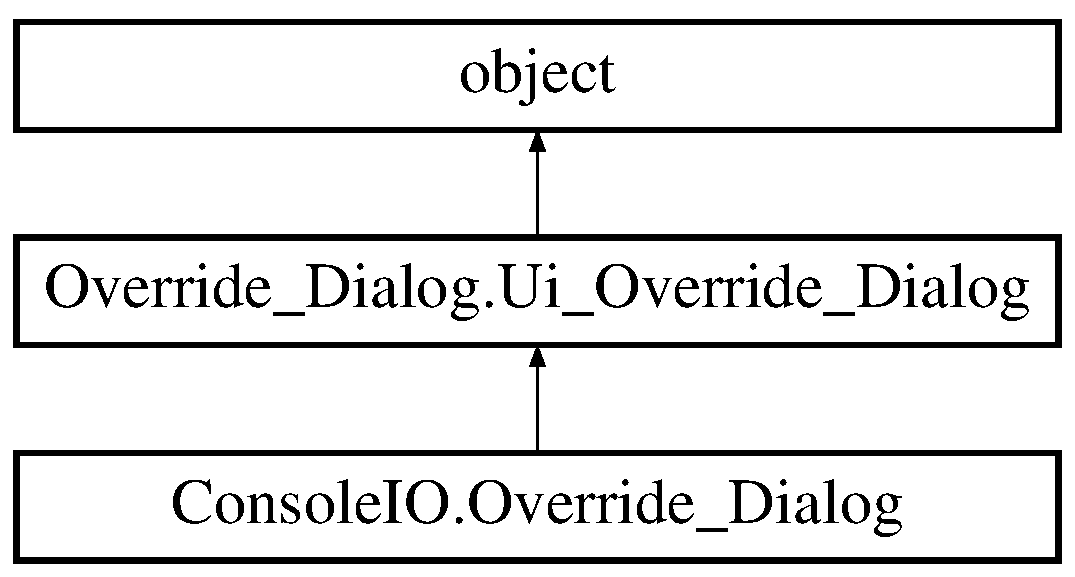
\includegraphics[height=3.000000cm]{classOverride__Dialog_1_1Ui__Override__Dialog}
\end{center}
\end{figure}
\subsection*{Public Member Functions}
\begin{DoxyCompactItemize}
\item 
\hypertarget{classOverride__Dialog_1_1Ui__Override__Dialog_a3bbcb40810b6afaf62c8c5df2d567268}{def {\bfseries setup\-Ui}}\label{classOverride__Dialog_1_1Ui__Override__Dialog_a3bbcb40810b6afaf62c8c5df2d567268}

\item 
\hypertarget{classOverride__Dialog_1_1Ui__Override__Dialog_a9d3be752381f7d1c2015b3a32f9e6a59}{def {\bfseries retranslate\-Ui}}\label{classOverride__Dialog_1_1Ui__Override__Dialog_a9d3be752381f7d1c2015b3a32f9e6a59}

\end{DoxyCompactItemize}
\subsection*{Public Attributes}
\begin{DoxyCompactItemize}
\item 
\hypertarget{classOverride__Dialog_1_1Ui__Override__Dialog_a3a70416e65bf2f2e266b66479a60bafb}{{\bfseries override\-\_\-constraint\-\_\-message\-\_\-label}}\label{classOverride__Dialog_1_1Ui__Override__Dialog_a3a70416e65bf2f2e266b66479a60bafb}

\item 
\hypertarget{classOverride__Dialog_1_1Ui__Override__Dialog_a93ffe5d03193b6c015ee6e9d1468238a}{{\bfseries override\-\_\-message\-\_\-label\-\_\-1}}\label{classOverride__Dialog_1_1Ui__Override__Dialog_a93ffe5d03193b6c015ee6e9d1468238a}

\item 
\hypertarget{classOverride__Dialog_1_1Ui__Override__Dialog_ae0f8a6fa2b82197fad83e4bb8e1d2aea}{{\bfseries override\-\_\-message\-\_\-label\-\_\-2}}\label{classOverride__Dialog_1_1Ui__Override__Dialog_ae0f8a6fa2b82197fad83e4bb8e1d2aea}

\item 
\hypertarget{classOverride__Dialog_1_1Ui__Override__Dialog_a194eaea83a5fad0ed64bae1cb48493a2}{{\bfseries override\-\_\-yes\-\_\-button}}\label{classOverride__Dialog_1_1Ui__Override__Dialog_a194eaea83a5fad0ed64bae1cb48493a2}

\item 
\hypertarget{classOverride__Dialog_1_1Ui__Override__Dialog_a1284c82be077bfe864987ec1c84f1d18}{{\bfseries override\-\_\-no\-\_\-button}}\label{classOverride__Dialog_1_1Ui__Override__Dialog_a1284c82be077bfe864987ec1c84f1d18}

\end{DoxyCompactItemize}


The documentation for this class was generated from the following file\-:\begin{DoxyCompactItemize}
\item 
Override\-\_\-\-Dialog.\-py\end{DoxyCompactItemize}

%--- End generated contents ---

% Index
\newpage
\phantomsection
\addcontentsline{toc}{chapter}{Index}
\printindex

\end{document}
